\documentclass[letterpaper]{article}
\usepackage[square,sort,comma,numbers]{natbib}
\usepackage{array}
%====================================================================%
../../../../tex/scufftex.tex

\newcommand\supsstar[1]{^{\hbox{\scriptsize{#1}}*}}
\newcommand\suptstar[1]{^{\hbox{\scriptsize{#1}}*}}
\newcommand{\iD}{_{i\text{\tiny D}}}
\newcommand{\jS}{_{j\text{\tiny S}}}
\newcommand{\bbVInv}{\rotatebox[origin=c]{180}{$\mathbb{V}$}}
\newcommand{\vbVInv}{\rotatebox[origin=c]{180}{$\vb{V}$}}

\newcommand{\OP}{\vb O\sups{power}}
\newcommand{\OG}{\overline{G}}
\newcommand{\SG}{\overline{\vb G}}
\newcommand{\IF}{^{i\text{\scriptsize F}}}
\newcommand{\IT}{^{i\text{\scriptsize T}}}
\newcommand{\lm}{_{\ell m}}
\newcommand{\lmp}{_{\ell^\prime m^\prime}}
\newcommand{\OutD}{^{\hbox{\scriptsize{out}}\dagger}}

\renewcommand{\hslash}{\,\backslash\hspace{-0.06in}h}
\newcommand{\jslash}{\backslash\hspace{-0.05in}j}
\newcommand{\RBar}{\overline{R}}
\newcommand{\RSlash}{\backslash\hspace{-0.08in}R}

\newcommand{\regstar}{^{\hbox{\scriptsize reg}*}}

\graphicspath{{figures/}}

%------------------------------------------------------------
%------------------------------------------------------------
%- Special commands for this document -----------------------
%------------------------------------------------------------
%------------------------------------------------------------

%------------------------------------------------------------
%------------------------------------------------------------
%- Document header  -----------------------------------------
%------------------------------------------------------------
%------------------------------------------------------------
\title {Electromagnetism in the Spherical-Wave Basis: \\
        {\large A (Somewhat Random) Compendium of Reference Formulas}
       }
\author {Homer Reid}
\date {August 1, 2016}

%------------------------------------------------------------
%------------------------------------------------------------
%- Start of actual document
%------------------------------------------------------------
%------------------------------------------------------------

\begin{document}
\pagestyle{myheadings}
\markright{Homer Reid: E\&M in the Spherical-Wave Basis}
\maketitle

\begin{abstract}
This memo consolidates and collects for reference
a somewhat random hodgepodge of formulas and results
in the spherical-wave approach to electromagnetism
that I have found useful over the years in developing
and testing {\sc scuff-em} and {\sc buff-em}.
\end{abstract}

\tableofcontents

%%%%%%%%%%%%%%%%%%%%%%%%%%%%%%%%%%%%%%%%%%%%%%%%%%%%%%%%%%%%%%%%%%%%%%
%%%%%%%%%%%%%%%%%%%%%%%%%%%%%%%%%%%%%%%%%%%%%%%%%%%%%%%%%%%%%%%%%%%%%%
%%%%%%%%%%%%%%%%%%%%%%%%%%%%%%%%%%%%%%%%%%%%%%%%%%%%%%%%%%%%%%%%%%%%%%
\newpage
\section{Vector Spherical Wave Solutions to Maxwell's Equations}
\label{SphericalWaveSection}

Many authors define pairs of three-vector-valued functions
$\{\vb M_{\ell m}(\vb x), \vb N_{\ell m}(\vb x)\}$
describing exact solutions of the source-free 
Maxwell's equations---namely, the vector Helmholtz equation
plus the divergence-free condition---in spherical coordinates for 
a homogeneous medium with wavenumber $k$, i.e.
%====================================================================%
\numeq{VectorHelmholtz}
{ \Big[\nabla \times \nabla \times - k^2 \Big]
  \left\{\begin{array}{c} \vb M_{\ell m} \\ \vb N_{\ell m}\end{array}\right\} = 0,
  \qquad
  \nabla \cdot
  \left\{\begin{array}{c} \vb M_{\ell m} \\ \vb N_{\ell m}\end{array}\right\} = 0.
}
%====================================================================%
In some cases, the set $\{\vb M, \vb N\}_{\ell m}$ is augmented to
include a third function $\{\vb L_{\ell m}\}$ that satisfies
the vector Helmholtz equation but is now \textit{curl-}free
(and not divergenceless):
%====================================================================%
\numeq{LDef}
{ \Big[\nabla \times \nabla \times - k^2 \Big]
  \vb  L_{\ell m}=0,
  \qquad
  \nabla \times \vb L_{\ell m}=0.
}
%====================================================================%
The function $\vb L_{\ell m}$ is not a solution of Maxwell's equations
and is never 
needed in a basis of expansion functions for \textit{fields},
but must be retained in a basis for expanding \textit{currents}
in inhomogeneous and/or anisotropic media.

In all cases, the $\{\vb M, \vb N, \vb L\}$
functions involve spherical Bessel functions and
spherical harmonics, but the precise definitions (including
sign conventions and normalization factors) vary from author
to author. In this section I set down the particular
conventions that I use. In the next section I give
explicit closed-form expressions for small $\ell$.

\paragraph{Vector spherical harmonics}
%====================================================================%
\begin{align*}
  \vb X\lm(\theta, \varphi) 
&\equiv \frac{i}{\sqrt{\ell(\ell+1)}}\nabla \times 
     \Big\{Y\lm(\theta, \varphi) \vb r\Big\}
\\
  \vb Z\lm(\theta, \varphi) &\equiv \vbhat{r} \times \vb X\lm(\theta, \varphi)
\end{align*}
%====================================================================%

\noindent More explicitly, the components of $\vb X$ and $\vb Z$ are
%====================================================================%
\begin{align*}
\vb X\lm(\theta, \phi) 
&= 
   \frac{i}{\sqrt{\ell(\ell+1)}}
   \left[  \frac{im}{\sin\theta}Y_{\ell m} \vbhatt{\theta}
           -\pard{Y_{\ell m}}{\theta}\vbhatt{\varphi}
   \right]
\\
\vb Z\lm(\theta, \phi) 
&=
   \frac{i}{\sqrt{\ell(\ell+1)}}
   \left[   \pard{Y_{\ell m}}{\theta}\vbhatt{\theta}
           +\frac{im}{\sin\theta}Y_{\ell m} \vbhatt{\varphi}
   \right].
\end{align*}
%====================================================================%
These are orthonormal in the sense that 
%====================================================================%
$$ \inp{\vb X}{\vb X}= \inp{\vb Z}{\vb Z}=1,
   \quad \inp{\vb X}{\vb Z}=0
$$
%====================================================================%
where the inner product is
%====================================================================%
$$
   \inp{\vb F}{\vb G}\equiv \int \, \vb F^* \cdot \vb G \, d\Omega
   = \int_0^\pi \, \int_0^{2\pi} \, 
     \vb F^*(\theta,\varphi)\cdot \vb G(\theta, \varphi)\,\sin\theta\,d\varphi\,d\theta
$$
%====================================================================%

Their divergences are:
%====================================================================%
\begin{subequations}
\begin{align}
\nabla \cdot \vb X\lm
 &=-\frac{m\cot\theta\csc\theta Y\lm(\theta,\varphi)}
         {r\sqrt{\ell(\ell+1)}}
\\
\nabla \cdot \vb Z\lm
 &= \frac{i\cot\theta}{r \sqrt{\ell(\ell+1)}}
    \Big[ m\cot\theta Y\lm(\theta, \varphi)
          + \xi\lm e^{-i\varphi}Y_{\ell,m+1}(\theta,\varphi)
    \Big]
\\
\xi\lm&\equiv\sqrt\frac{ (\ell-m)! (\ell+m+1)!}{(\ell-m-1)!(\ell+m)!}
\end{align}
\label{XZDivergences}
\end{subequations}
%====================================================================%

\paragraph{Radial functions}
%====================================================================%
\begin{align*}
 R_\ell \sups{outgoing}(kr)  &\equiv h^{(1)}_\ell(kr) \\
 R_\ell \sups{incoming}(kr)  &\equiv h^{(2)}_\ell(kr) \\
 R_\ell \sups{regular}(kr)   &\equiv j_\ell(kr).
\end{align*}
%====================================================================%
I also define the shorthand symbols
%====================================================================%
$$ \RBar_\ell(kr)
   \equiv 
   \frac{1}{kr}R_\ell(kr) + R^\prime_\ell(kr)
   \qquad
   \RSlash_\ell(kr) \equiv -\frac{\sqrt{l(l+1)}}{kr} R_\ell(kr)
$$
where $R^\prime_\ell(kr) = \left|\frac{d}{dz}R_\ell(z)\right|_{z=kr}.$
%====================================================================%

\paragraph{Scalar Helmholtz solutions}

%====================================================================%
$$ \Big[ \nabla^2 + k^2\Big]\psi\lm(\vb r) = 0
   \whereupon
   \psi\lm(r,\theta,\varphi)=R_\ell(kr) Y_{\ell m}(\theta,\varphi)
$$
%====================================================================%
where $R_\ell$ is one of the radial functions defined above.

\paragraph{Vector spherical wave functions}

%====================================================================%
\numeq{MNLDef}
{
 \begin{array}{>{\displaystyle}lc>{\displaystyle}lc>{\displaystyle}l}
 \vb M\lm(k; \vb r) 
 &\equiv&\frac{i}{\sqrt{\ell(\ell+1)}}\nabla\Big\{\psi\lm \vb r\Big\}
 &=&R_\ell(kr) \vb X\lm(\Omega) 
\\[8pt]
%--------------------------------------------------------------------%
 \vb N\lm(k; \vb r) 
 &\equiv&-\frac{1}{ik}\nabla \times \vb M\lm
 &=&
i\RBar_\ell(kr) \vb Z\lm(\Omega) + \RSlash_\ell(kr) Y\lm(\Omega) \vbhat{r} 
\\[8pt]
%--------------------------------------------------------------------%
 \vb L\lm(k; \vb r)
 &\equiv&\frac{1}{k\sqrt{\ell(\ell+1)}}\nabla \psi\lm
 &=& -i\frac{R_\ell(kr)}{kr}\vb Z\lm(\Omega)
    +\frac{1}{\sqrt{\ell(\ell+1)}}R^\prime_\ell(kr) Y\lm(\Omega)\vbhat{r}
 \end{array}
}
%====================================================================%
$$ \vb L_{00}(k; \vb r) = \frac{R^\prime_0(kr)}{\sqrt{4\pi}}\vbhat{r}$$

\paragraph{Curl Identities}

$$ \nabla \times \vb M = -ik\vb N, \qquad
   \nabla \times \vb N = +ik\vb M.
$$

\paragraph{General solution of source-free Maxwell equations}

The general solution of Maxwell's equations in a source-free
medium with relative material properties $\epsilon^r, \mu^r$ 
then reads
%====================================================================%
\begin{subequations}
\begin{align}
 \vb E(\vb x)
 &= \hphantom{\frac{1}{Z_0 Z^r}} \sum_\alpha 
     \Big\{ \vb A_\alpha \vb M_\alpha(k; \vb r)
           +\vb B_\alpha \vb N_\alpha(k; \vb r)
     \Big\} 
\\
 \vb H(\vb x)
 &= \frac{1}{Z_0 Z^r} \sum_\alpha 
     \Big\{ \vb B_\alpha \vb M_\alpha(k; \vb r)
           -\vb A_\alpha \vb N_\alpha(k; \vb r)
     \Big\} 
\end{align}
\label{EHExpansion}%%%%
\end{subequations}
%====================================================================%
where $k=\sqrt{\epsilon_0 \epsilon^r \mu_0 \mu^r}\cdot \omega$
is the photon wavenumber in the medium,
$Z_0=\sqrt{\mu_0/\epsilon_0}\sim 377\,\Omega$ is the impedance
of vacuum,
$Z^r=\sqrt{\mu^r/\epsilon^r}$ is the relative wave impedance
of the medium, and we must choose the $\vb M, \vb N$ 
functions to be regular, incoming, or outgoing depending
on the physical conditions of the problem.

\paragraph{Unified notation for $\vb M, \vb N$ waves}

I will use the symbol $\bmc W_\alpha$ to refer
collectively to $\vb M$ and $\vb N$ waves;
here\footnote{With this notation I am committing the
faux pas of using the same symbol $\alpha$ for
the two-fold compound index $(\ell m)$ in (\ref{EHExpansion})
and the three-fold compound index $(\ell m P)$ in
(\ref{EHExpansion2}), but \textit{whaddya gonna do.}}
$\alpha=(\ell m P)$ is a compound index
with $P=\{M,N\}$ identifying the polarization.
With this notation, expansions such as (\ref{EHExpansion})
read
%====================================================================%
\numeq{EHExpansion2}
{\vb E = \sum_\alpha C_\alpha \bmc W_\alpha, \qquad
   \vb H = 
   \frac{1}{Z_0Z^r}\sum_\alpha C_\alpha \sigma_{\alpha} \bmc W_{\overline{\alpha}}
}
%====================================================================%
where 
$$ \sum_\alpha\{\cdots\} 
   = 
   \sum_{\ell}\sum_{m=-\ell}^\ell \sum_{P\in \{M,N\}} \{\cdots\}
$$
%====================================================================%
and 
$$
   \overline{\ell m M} = \ell m N, \qquad
   \overline{\ell m N} = \ell m M, \qquad
   \sigma_{\ell m M}=+1, \qquad
   \sigma_{\ell m N}=-1.
$$
%====================================================================%
\paragraph{Spherical-wave expansion of dyadic Green's function}

Let $\mb G(k; \vb r)$ and $\mb C(k; \vb r)$ be the usual
homogeneous dyadic Green's functions, with Cartesian components
%====================================================================%
\numeq{GCDef}
{
 \mb G_{ij}(k; \vb r)
=\Big( \delta_{ij} + \frac{1}{k^2}\partial_i \partial_j\Big)
  \frac{e^{ik|\vb r|}}{4\pi|\vb r|},
  \qquad
\mb C_{ij}(k, \vb r) = +\frac{1}{ik} \varepsilon_{ijl} 
                         \partial_l \mb G(k, \vb r)
}
%====================================================================%
Then have the spherical-wave expansion
%====================================================================%
\begin{subequations}
\begin{align}
  \mb G(\vb x, \vb x^\prime)
&= -\frac{1}{k^2}\delta(\vb x-\vb x^\prime)\vbhat{r}\vbhat{r}^\prime
     + ik \sum_\alpha 
          \bmc W_\alpha\sups{out}(\vb x_>)
          \bmc W_\alpha\sups{reg}(\vb x_<),
\\
\mb C(\vb x, \vb x^\prime)
&= ik\sum_{\alpha} \sigma_\alpha
   \begin{dcases}
     \bmc W_{\overline \alpha}\sups{out}(\vb x)
     \bmc W_{\alpha}\sups{reg}(\vb x^\prime), \qquad |\vb x|>|\vb x^\prime|,
\\
     \bmc W_{\overline \alpha}\sups{out}(\vb x^\prime)
     \bmc W_{\alpha}\sups{reg}(\vb x), \qquad |\vb x|<|\vb x^\prime|
     \end{dcases} 
\end{align}
\label{GCExpansions}
\end{subequations}
%====================================================================%

%%%%%%%%%%%%%%%%%%%%%%%%%%%%%%%%%%%%%%%%%%%%%%%%%%%%%%%%%%%%%%%%%%%%%%
%%%%%%%%%%%%%%%%%%%%%%%%%%%%%%%%%%%%%%%%%%%%%%%%%%%%%%%%%%%%%%%%%%%%%%
%%%%%%%%%%%%%%%%%%%%%%%%%%%%%%%%%%%%%%%%%%%%%%%%%%%%%%%%%%%%%%%%%%%%%%
\newpage
\section{Explicit expression for small $\ell$}
\label{ExplicitExpressionSection}

\paragraph{The first few radial functions}

%====================================================================%
$$\begin{array}{lclclcl}
%--------------------------------------------------------------------%
 R\sups{regular}_0(x) 
&=&
 \displaystyle{ \frac{\sin x}{x}}
&\qquad&
 \displaystyle{ \RBar\sups{regular}_0(x)  }
&=&
 \displaystyle{ \frac{\cos x}{x}
              }
\\[10pt]
%--------------------------------------------------------------------%
 R\sups{outgoing}_0(x) 
&=&
 \displaystyle{ -i\frac{e^{ix}}{x}}
&\qquad&
 \displaystyle{ \RBar\sups{outgoing}_0(x) }
&=&
 \displaystyle{ \frac{e^{ix}}{x}}
\\
%--------------------------------------------------------------------%
 R\sups{regular}_1(x) 
&=&
 \displaystyle{ \frac{\sin x - x\cos x}{x^2} }
&\qquad&
 \displaystyle{ \RBar\sups{regular}_1(x)  }
&=&
 \displaystyle{ \frac{x\cos x + (x^2-1)\sin x}{x^3}
              }
\\[10pt]
%--------------------------------------------------------------------%
 R\sups{outgoing}_1(x) 
&=&
 \displaystyle{ -\frac{ie^{ix}}{x^2}\big(1-ix\big)}
&\qquad&
 \displaystyle{ \RBar\sups{outgoing}_1(x) }
&=&
 \displaystyle{ \frac{ie^{ix}}{x^3}\big(1-ix-x^2\big) }
\end{array}$$
%====================================================================%

\paragraph{The first few regular functions}

In what follows, the $\zeta_n$ are dimensionless sinusoidal functions:
%====================================================================%
\begin{align*}
 \zeta_1(x) &= \sin x - x \cos x \\
 \zeta_2(x) &= (1-x^2)\sin x - x \cos x
\end{align*}
%====================================================================%

%====================================================================%
\begin{align*}
 \vb L\sups{regular}_{00}(\vb r)
  &=-\frac{\zeta_1(kr)}{4\pi(kr)^2}
    \left(\begin{array}{c}
    1                 \\
    0                 \\
    0
    \end{array}\right)
\\
%--------------------------------------------------------------------%
&\xrightarrow{k\to 0}
 \frac{kr}{6\sqrt\pi}
    \left(\begin{array}{c} 1 \\ 0 \\ 0 \end{array}\right)
\\[8pt]
%--------------------------------------------------------------------%
 \vb M\sups{regular}_{1,\pm 1}(\vb r)
  &=\sqrt\frac{3}{16\pi}\sbf{\zeta_1(kr)}{(kr)^2} e^{\pm i\varphi}
    \left(\begin{array}{c}
    0                 \\
    1                 \\
    \pm i\cos \theta
    \end{array}\right)
\\[5pt]
%--------------------------------------------------------------------%
 &\xrightarrow{k\to 0}
    \frac{kr}{4\sqrt{3\pi}} e^{\pm i\varphi}
    \left(\begin{array}{c}
    0                 \\
    1                 \\
    \pm i\cos \theta
    \end{array}\right)
\\[8pt]
%--------------------------------------------------------------------%
 \vb M\sups{regular}_{1,0}(\vb r)
  &=i\sqrt\frac{3}{2\pi}\pf{ \sin kr - kr\cos kr}{(kr)^2}   
    \left(\begin{array}{c}
    0                 \\
    0                 \\
    \sin\theta
    \end{array}\right)
\\[5pt]
%--------------------------------------------------------------------%
 &\xrightarrow{k\to 0}
    i\sqrt\frac{3}{8\pi}\sbf{\zeta(kr)}{(kr)^2}
    \left(\begin{array}{c}
    0                 \\
    0                 \\
    \sin\theta
    \end{array}\right)
\\[5pt]
%--------------------------------------------------------------------%
 \vb N\sups{regular}_{1,\pm 1}(\vb r)
  &=\sqrt\frac{3}{16\pi}\sbf{1}{(kr)^3} e^{\pm i\varphi}
    \left(\begin{array}{c}
    \pm 2\zeta_1(kr) \sin \theta \\
    \mp\zeta_2(kr) \cos \theta \\
    -i\zeta_2(kr)
    \end{array}\right)
\\[5pt]
%--------------------------------------------------------------------%
&\xrightarrow{k\to 0}
 \sqrt\frac{e^{\pm i\varphi}}{12\pi}
    \left(\begin{array}{c}
    \pm\sin\theta \\
    \pm\cos\theta \\
    i
    \end{array}\right)
\\[8pt]
%--------------------------------------------------------------------%
 \vb N\sups{regular}_{1,0}(\vb r)
  &=\sqrt\frac{3}{8\pi}\sbf{1}{(kr)^3}
    \left(\begin{array}{c}
    -2\zeta_1(kr)\cos\theta \\
    -\zeta_2(kr)\sin\theta  \\
    0                
    \end{array}\right)
\\[5pt]
%--------------------------------------------------------------------%
&\xrightarrow{k\to 0}
    \frac{1}{\sqrt{6\pi}}
    \left(\begin{array}{c}
    -\cos\theta \\
    \sin\theta \\
    0
    \end{array}\right)
=-\frac{1}{\sqrt{6\pi}}\vbhat{z}
%--------------------------------------------------------------------%
\end{align*}
%====================================================================%

\paragraph{The first few outgoing functions}

In what follows, the $Q_n$ are dimensionless polynomial factors:
%====================================================================%
\begin{align*}
 Q_1(x) &= 1-x \\
 Q_{2a}(x) &= 1-x+x^2 \\
 Q_{2b}(x) &= 3-3x+x^2 \\
 Q_3(x) &= 6-6x+3x^2-x^3
\end{align*}
%====================================================================%
\begin{align*}
 \vb M\sups{outgoing}_{1,\pm 1}(\vb r)
  &=\sqrt\frac{3}{16\pi}\pf{e^{ikr}}{k^2 r^2} e^{\pm i\phi}
    \left(\begin{array}{c}
    0          \\
    -iQ_1(ikr) \\
    \pm Q_1(ikr) \cos\theta 
    \end{array}\right)
\\[5pt]
%--------------------------------------------------------------------%
 \vb M\sups{outgoing}_{1,0}(\vb r)
  &=\sqrt\frac{3}{8\pi}\pf{e^{ikr}}{k^2 r^2}
    \left(\begin{array}{c}
    0       \\
    0       \\
    Q_1(ikr) \sin\theta 
    \end{array}\right)
\\
%--------------------------------------------------------------------%
 \vb N\sups{outgoing}_{1,\pm 1}(\vb r)
  &=\sqrt\frac{3}{16\pi}\pf{e^{ikr}}{k^3 r^3} e^{\pm i\phi}
    \left(\begin{array}{c}
    \mp -2(ikr)Q_1(ikr)\sin \theta   \\
    \pm iQ_{2a}(ikr) \cos\theta      \\
    -Q_{2a}(ikr)
    \end{array}\right)
\\
%--------------------------------------------------------------------%
 \vb N\sups{outgoing}_{1,0}(\vb r)
  &=\sqrt\frac{3}{8\pi}\pf{e^{ikr}}{k^3 r^3}
    \left(\begin{array}{c}
    2iQ_1(ikr)\cos \theta		\\
    +iQ_{2a}(ikr)\sin\theta	\\
    0
    \end{array}\right)
\\[5pt]
%--------------------------------------------------------------------%
 \vb M\sups{outgoing}_{2,\pm 2}(\vb r)
  &=\sqrt\frac{5}{16\pi}\pf{e^{ikr}}{k^3 r^3} e^{\pm 2i\phi}
    \left(\begin{array}{c}
    0 				  \\
   \pm  iQ_{2b}(ikr)\sin\theta	  \\
    -Q_{2b}(ikr)\cos\theta\sin\theta
    \end{array}\right)
\\
%--------------------------------------------------------------------%
 \vb M\sups{outgoing}_{2,\pm 1}(\vb r)
  &=\sqrt\frac{5}{16\pi}\pf{e^{ikr}}{k^3 r^3} e^{\pm i\phi}
    \left(\begin{array}{c}
    0                            \\
    -iQ_{2b}(ikr)\cos\theta  \\
    \pm Q_{2b}(ikr)\cos 2\theta
    \end{array}\right)
\\
%--------------------------------------------------------------------%
 \vb M\sups{outgoing}_{2,0}(\vb r)
  &=\sqrt\frac{15}{8\pi}\pf{e^{ikr}}{k^3 r^3}
    \left(\begin{array}{c}
    0 \\ 
    0 \\ 
    -Q_{2b}(ikr)\cos \theta \sin\theta
    \end{array}\right)
\\[5pt]
%--------------------------------------------------------------------%
 \vb N\sups{outgoing}_{2,\pm 2}(\vb r)
  &=\sqrt\frac{5}{16\pi}\pf{e^{ikr}}{k^4 r^4} e^{\pm 2i\phi}
    \left(\begin{array}{c}
   3iQ_{2b}(ikr) \sin^2 \theta                          \\
   -iQ_3(ikr) \cos\theta \sin\theta   \\
   \pm Q_3(ikr) \sin\theta 
    \end{array}\right)
\\
%--------------------------------------------------------------------%
 \vb N\sups{outgoing}_{2,\pm 1}(\vb r)
  &=\sqrt\frac{5}{16\pi}\pf{e^{ikr}}{k^4 r^4} e^{\pm i\phi}
    \left(\begin{array}{c}
   \mp 3iQ_{2b}(ikr) \sin 2\theta               \\
   \pm iQ_3(ikr) \cos 2\theta  \\
   -Q_3(ikr) \cos\theta
    \end{array}\right)
\\
%--------------------------------------------------------------------%
 \vb N\sups{outgoing}_{2,0}(\vb r)
  &=\sqrt\frac{15}{8\pi}\pf{e^{ikr}}{k^4 r^4}
    \left(\begin{array}{c}
   iQ_{2b}(ikr)(3\cos^2 \theta -1)                    \\
   iQ_3(ikr) \cos \theta \sin\theta \\
   0
    \end{array}\right).
\end{align*}

%%%%%%%%%%%%%%%%%%%%%%%%%%%%%%%%%%%%%%%%%%%%%%%%%%%%%%%%%%%%%%%%%%%%%%
%%%%%%%%%%%%%%%%%%%%%%%%%%%%%%%%%%%%%%%%%%%%%%%%%%%%%%%%%%%%%%%%%%%%%%
%%%%%%%%%%%%%%%%%%%%%%%%%%%%%%%%%%%%%%%%%%%%%%%%%%%%%%%%%%%%%%%%%%%%%%
\newpage
\section{Translation matrices}
\label{TranslationMatrixSection}

Translation matrices arise when we want to evaluate the fields
produced by sources not located at the origin. 

\paragraph{Scalar case}
Although we don't need it for electromagnetism problems,
the scalar-wave analog of (\ref{MNLDef}) is
%%%%%%%%%%%%%%%%%%%%%%%%%%%%%%%%%%%%%%%%%%%%%%%%%%%%%%%%%%%%%%%%%%%%%%
$$ \psi\lm(\vb x) = R_\ell(kr)Y\lm(\theta,\phi)$$
%%%%%%%%%%%%%%%%%%%%%%%%%%%%%%%%%%%%%%%%%%%%%%%%%%%%%%%%%%%%%%%%%%%%%%
or, more specifically,
%%%%%%%%%%%%%%%%%%%%%%%%%%%%%%%%%%%%%%%%%%%%%%%%%%%%%%%%%%%%%%%%%%%%%%
$$ \psi\lm\sups{out}(\vb x) = R_\ell\sups{out}(kr)Y\lm(\theta,\phi),
   \qquad
   \psi\lm\sups{reg}(\vb x) = R_\ell\sups{reg}(kr)Y\lm(\theta,\phi)
$$
%%%%%%%%%%%%%%%%%%%%%%%%%%%%%%%%%%%%%%%%%%%%%%%%%%%%%%%%%%%%%%%%%%%%%%
Now consider a point source at $\vb x\supt{S}$ whose fields we wish
to evaluate at an evaluation (``destination'') point $\vb x\supt{D}$,
using a basis of spherical waves centered at an origin $\vb x\supt{O}$.
Then waves emitted by the source, which appear to be outgoing in a
coordinate system centered at $\vb x\supt{S}$, can be described
as superpositions of regular waves in a coordinate system
centered at $\vb x\supt{O}$:
%%%%%%%%%%%%%%%%%%%%%%%%%%%%%%%%%%%%%%%%%%%%%%%%%%%%%%%%%%%%%%%%%%%%%%
\numeq{ScalarTranslationFormula}
{ \psi\sups{out}_\alpha\big(\vb x\supt{D}-\vb x\supt{S}\big)
   =\sum_\beta A_{\alpha\beta}\big(k; \vb x\supt{S} - \vb x\supt{O}\big)
               \psi\sups{reg}_\beta\big( \vb x\supt{D}-\vb x\supt{O}\big)
}
where $\alpha,\beta$ are compound indices 
(i.e. $\alpha=\{\ell_\alpha, m_\alpha\}$) and 
%%%%%%%%%%%%%%%%%%%%%%%%%%%%%%%%%%%%%%%%%%%%%%%%%%%%%%%%%%%%%%%%%%%%%%
\begin{align*}
 A_{\alpha\beta}(k, \vb L)
&=4\pi 
  \sum_\gamma i^{(\ell_\alpha - \ell_\beta + \ell_\gamma)}
  a_{\alpha\gamma\beta} 
  \psi\sups{out}_\gamma(\vb L)
\\
a_{\alpha\beta\gamma}
&=\int Y_\alpha(\Omega) Y^*_\beta(\Omega) Y^*_\gamma(\Omega) \, d\Omega
\\
&=(-1)^{m_\alpha}
  \sqrt\frac{ (2\ell_\alpha+1)(2\ell_\beta+1) (2\ell_\gamma+1)}
            {4\pi}
  \left(\begin{array}{ccc} 
        \ell_\alpha & \ell_\beta & \ell_\gamma \\ 0 & 0 & 0 
        \end{array}\right)
  \left(\begin{array}{ccc} 
        \ell_\alpha & \ell_\beta & \ell_\gamma \\ 
          -m_\alpha & m_\beta    & m_\gamma
        \end{array}\right).
\end{align*}
%%%%%%%%%%%%%%%%%%%%%%%%%%%%%%%%%%%%%%%%%%%%%%%%%%%%%%%%%%%%%%%%%%%%%%

\paragraph{Vector case}

%%%%%%%%%%%%%%%%%%%%%%%%%%%%%%%%%%%%%%%%%%%%%%%%%%%%%%%%%%%%%%%%%%%%%%
\begin{align*}
 \left(\begin{array}{c}
   \vb M \\ \vb N
 \end{array}\right)\sups{out}_\alpha
&= 
 \sum_{\beta}
 \left(\begin{array}{cc}
   \vb B & \vb C \\ 
  -\vb C & \vb B
 \end{array}\right)_{\alpha\beta} 
 \left(\begin{array}{c}
   \vb M \\ \vb N 
 \end{array}\right)\sups{reg}_\beta
\end{align*}
%%%%%%%%%%%%%%%%%%%%%%%%%%%%%%%%%%%%%%%%%%%%%%%%%%%%%%%%%%%%%%%%%%%%%%

%%%%%%%%%%%%%%%%%%%%%%%%%%%%%%%%%%%%%%%%%%%%%%%%%%%%%%%%%%%%%%%%%%%%%%
\begin{align*}
 B_{\alpha\beta}(k, \vb L)
&=4\pi 
  \sum_\gamma i^{(\ell_\alpha - \ell_\beta + \ell_\gamma)}
  \left[\frac{\ell_\alpha(\ell_\alpha + 1) + \ell_\beta(\ell_\beta + 1) 
               -\ell_\gamma(\ell_\gamma+ 1)
             }
             {2\sqrt{\ell_\alpha(\ell_\alpha+1)\ell_\beta (\ell_\beta+1)}}
  \right]
  a_{\alpha\gamma\beta} 
  \psi\sups{out}_\gamma(\vb L)
\\
 C_{\alpha\beta}(k, \vb L)
&=-\frac{k}{\sqrt{\ell_\alpha(\ell_\alpha+1)\ell_\beta(\ell_\beta+1)}}
   \left[ \frac{\lambda_+}{2}\big(L_x - iL_y\big)A_{\alpha_+, \beta} 
         +\frac{\lambda_-}{2}\big(L_x + iL_y\big)A_{\alpha_-, \beta} 
         +           m_\alpha L_z A_{\alpha, \beta} 
   \right]
\end{align*}
$$ \lambda_\pm = \sqrt{ (\ell_\alpha \mp \ell_\beta)
                        (\ell_\alpha \pm \ell_\beta+1)
                      },
   \qquad
   \alpha_\pm = \{\ell_\alpha, m_\alpha \pm 1\}
$$

%%%%%%%%%%%%%%%%%%%%%%%%%%%%%%%%%%%%%%%%%%%%%%%%%%%%%%%%%%%%%%%%%%%%%%
%%%%%%%%%%%%%%%%%%%%%%%%%%%%%%%%%%%%%%%%%%%%%%%%%%%%%%%%%%%%%%%%%%%%%%
%%%%%%%%%%%%%%%%%%%%%%%%%%%%%%%%%%%%%%%%%%%%%%%%%%%%%%%%%%%%%%%%%%%%%%
\newpage
\section{Spherical-wave expansion of incident fields}
\label{IncidentFieldSection}

\subsection{Plane waves}
\label{PlaneWaveSection}

For a scattering problem in which the incident field
is a $z$-directed plane wave, i.e.
%====================================================================%
$$
 \vb E\sups{inc}=\vb E_0e^{ik z}, \qquad 
 \vb H\sups{inc}=\frac{1}{Z_0}\vbhat{z}\times \vb E_0 e^{ik z}
$$
%====================================================================%
the spherical-wave expansion coefficients in (\ref{EHIncOutsideExpansion})
take the following forms for various possible polarizations:
%====================================================================%
$$\begin{array}{rclll}
\vb E_0 &=& \vbhat{x} + i\vbhat{y} 
 \quad &\text{(right circular polarization)}:
 \qquad &P\lm=\delta_{m,+1}P_\ell
\\[5pt]
\vb E_0 &=& \vbhat{x} - i\vbhat{y} 
 \quad &\text{(left circular polarization)}:
 \qquad &P\lm=\delta_{m,-1}P_\ell 
\\[3pt]
\vb E_0 &=& \vbhat{x}
 \quad &\text{(linear polarization)}:
 \qquad &P\lm=\frac{1}{2}\Big(\delta_{m,+1} + \delta_{m,-1}\Big)P_\ell 
\end{array}$$
%====================================================================%
where in all cases I have
%====================================================================%
$$ P_\ell = i^\ell \sqrt{4\pi(2\ell +1)}, \qquad  
   Q_{\ell, \pm 1} = \mp i P_\ell.
$$
%====================================================================%

%%%%%%%%%%%%%%%%%%%%%%%%%%%%%%%%%%%%%%%%%%%%%%%%%%%%%%%%%%%%%%%%%%%%%%
%%%%%%%%%%%%%%%%%%%%%%%%%%%%%%%%%%%%%%%%%%%%%%%%%%%%%%%%%%%%%%%%%%%%%%
%%%%%%%%%%%%%%%%%%%%%%%%%%%%%%%%%%%%%%%%%%%%%%%%%%%%%%%%%%%%%%%%%%%%%%
\subsection{Point sources at the origin}
\label{PointSourceAtOriginSection}

Let $\vb E(\vb x; \vb p)$ be the electric field
at evaluation point $\vb x$ due to an electric dipole
$\vb p$ at the origin. The spherical-wave expansion
of this field involves only $\vb N$-functions
with $\ell=1$, i.e.
%====================================================================%
$$ \vb E(\vb x; \vb p) = 
   \sum_{m=-1}^1 \xi_{1m}(\vb p) \vb N_{1m}\sups{outgoing}(\vb x)
$$
%====================================================================%
where the $\xi$ coefficients are
%====================================================================%
$$\begin{array}{clll}
\vb p=p_x \vbhat{x}
&\qquad\longrightarrow\qquad
&\displaystyle{
  \xi_{1,1}=-\xi_{1,-1}=\frac{i}{2}\frac{k^3}{\sqrt{3\pi}}\frac{p_x}{\epsilon},
              }
&\qquad\xi_{1,0}=0
\\[10pt]
\vb p=p_y \vbhat{y}
&\qquad\longrightarrow\qquad
&\displaystyle{
 \xi_{1,1}=+\xi_{1,-1}=\frac{1}{2}\frac{k^3}{\sqrt{3\pi}}\frac{p_y}{\epsilon}
              }
&\qquad\xi_{1,0}=0
\\[10pt]
\vb p=p_z \vbhat{z}
&\qquad\longrightarrow\qquad
&\displaystyle{
 \xi_{1,1}=\xi_{1,-1}=0, 
              } 
&\qquad \xi_{1,0} = 
  \displaystyle{ -\frac{ik^3}{\sqrt{6\pi}} \frac{p_z}{\epsilon} }
\end{array}$$
%====================================================================%
Here $\epsilon=\epsilon_0\epsilon^r$ is the absolute permittivity
of the medium.

Similarly, the magnetic fields of a magnetic dipole $\vb m$ at the
origin are
$$ \vb H(\vb x; \vb m)=\sum_\alpha \wh{\xi}_\alpha(\vb m) \vb N\sups{outgoing}_\alpha(\vb x)
$$
where the $\wh{\xi}$ coefficients are the same as the
$\xi$ coefficients above with the replacement
$\frac{p}{\epsilon} \to \frac{m}{\mu}.$

%=================================================
%=================================================
%=================================================
\subsection{Point sources not at the origin}
\label{PointSourceSection}

The fields of point sources \textit{not} at the
origin may be obtained by applying the translation matrices
of Section \label{TranslationMatrixSection}
to the fields of Section \ref{PointSourceAtOriginSection}.
If the point source lies at $\vb x\supt{S}\ne 0$ (here ``S''
stands for ``source''), then 
its fields at destination point $\vb x\supt{D}$
read
%====================================================================%
\begin{subequations}
\begin{align}
 \vb E(\vb x\supt{D}; \vb x\supt{S}, \vb p)
   &= \sum_{\alpha\beta}
      \Big\{
       -\xi_\alpha C_{\alpha\beta}  \vb M_\beta\sups{regular}(\vb x\supt{D})
       +\xi_\alpha B_{\alpha\beta} \vb N_\beta\sups{regular}(\vb x\supt{D})
      \Big\}
\\
 \vb H(\vb x\supt{D}; \vb x\supt{S}, \vb p)
   &= \frac{1}{Z}\sum_{\alpha\beta}
                    \Big\{
         \xi_\alpha C_{\alpha\beta} \vb N_\beta\sups{regular}(\vb x\supt{D})
       + \xi_\alpha B_{\alpha\beta} \vb M_\beta\sups{regular}(\vb x\supt{D})
                    \Big\}
\\[10pt]
 \vb E(\vb x\supt{D}; \vb x\supt{S}, \vb m)
   &=-Z \sum_{\alpha\beta} \Big\{
        \wh{\xi}_\alpha B_{\alpha\beta} \vb M_\beta\sups{regular}(\vb x\supt{D})
       +\wh{\xi}_\alpha C_{\alpha\beta} \vb N_\beta\sups{regular}(\vb x\supt{D})
                    \Big\}
\\
 \vb H(\vb x\supt{D}; \vb x\supt{S}, \vb m)
   &= \sum_{\alpha\beta} \Big\{
       -\wh{\xi}_\alpha C_{\alpha\beta} \vb M_\beta\sups{regular}(\vb x\supt{D})
       +\wh{\xi}_\alpha B_{\alpha\beta} \vb N_\beta\sups{regular}(\vb x\supt{D})
                    \Big\}
\end{align}
\label{TranslatedPSFields}
\end{subequations}
%====================================================================%
Here $\{B,C\}_{\alpha\beta}$ are elements of the translation matrices
$\vb B(k,\vb x\supt{S}), \vb C(k,\vb x\supt{S}).$

Note that, for a given source point $\vb x\supt{S}$, I only have
to assemble the translation matrices $\vb B$ and $\vb C$ once
(at a given frequency), after which I can get the fields
at any number of destination points $\vb x\supt{D}$ from
equation (\ref{TranslatedPSFields}).


%%%%%%%%%%%%%%%%%%%%%%%%%%%%%%%%%%%%%%%%%%%%%%%%%%%%%%%%%%%%%%%%%%%%%%
%%%%%%%%%%%%%%%%%%%%%%%%%%%%%%%%%%%%%%%%%%%%%%%%%%%%%%%%%%%%%%%%%%%%%%
%%%%%%%%%%%%%%%%%%%%%%%%%%%%%%%%%%%%%%%%%%%%%%%%%%%%%%%%%%%%%%%%%%%%%%
\newpage
\section{Scattering from a homogeneous dielectric sphere}
\label{DielectricSphereScatteringSectionl}

I consider scattering from a single homogeneous sphere
with relative permittivity and permeability $\epsilon^r, \mu^r$
in vacuum
irradiated by spherical waves emanating from within our
outside the sphere.

Irrespective of the origin of the incident fields, 
the scattered fields inside and outside the sphere
take the form ($n=\sqrt{\epsilon^r \mu^r}, Z^r=\sqrt{\mu^r / \epsilon^r})$
%====================================================================%
\paragraph{Inside the sphere:} 
\begin{subequations}
\begin{align}
 \vb E\sups{scat}(\vb x)
 &=\hphantom{\frac{1}{Z_0 Z^r}}  \sum_\alpha 
     \Big\{ A_\alpha \vb M_\alpha\sups{reg}(nk_0; \vb r)
        +   B_\alpha \vb N_\alpha\sups{reg}(nk_0; \vb r)
     \Big\} 
\\
 \vb H\sups{scat}(\vb x)
 &= \frac{1}{Z_0 Z^r} \sum_\alpha 
     \Big\{ B_\alpha \vb M_\alpha\sups{reg}(nk_0; \vb r)
           -A_\alpha \vb N_\alpha\sups{reg}(nk_0; \vb r)
     \Big\} 
\end{align}
\label{EHScatInside}
\end{subequations}
\paragraph{Outside the sphere:} 
\begin{subequations}
\begin{align}
 \vb E\sups{scat}(\vb x)
 &=\hphantom{\frac{1}{Z_0}}  \sum_\alpha 
      \Big\{ C_\alpha \vb M_\alpha\sups{out}(k_0; \vb r)
            +D_\alpha \vb N_\alpha\sups{out}(k_0; \vb r)
      \Big\} 
\\
 \vb H\sups{scat}(\vb x)
 &=  \frac{1}{Z_0} \sum_\alpha 
     \Big\{ D_\alpha \vb M_\alpha\sups{out}(k_0; \vb r)
           -C_\alpha \vb N_\alpha\sups{out}(k_0; \vb r)
     \Big\} 
\end{align}
\label{EHScatOutside}%
\end{subequations}
%====================================================================%
The $\{A, B, C, D\}$ coefficients are proportional to the 
spherical-wave expansion coefficients of the incident fields,
with the proportionality constants determined by enforcing
continuity of the tangential components of the total 
fields $\{\vb E, \vb H\}\sups{tot}=
\{\vb E, \vb H\}\sups{inc}+
\{\vb E, \vb H\}\sups{scat}$
at $r=r_0$,
%====================================================================%
\begin{subequations}
\begin{align}
 \Big| \vbhat{r} \times \vb E\sups{tot} \Big|_{r\to r_0^+}
&=
 \Big| \vbhat{r} \times \vb E\sups{tot} \Big|_{r\to r_0^-}
\\[5pt]
 \Big| \vbhat{r} \times \vb H\sups{tot} \Big|_{r\to r_0^+}
&=
 \Big| \vbhat{r} \times \vb H\sups{tot} \Big|_{r\to r_0^-}
\end{align}
\label{EHMatching}%
\end{subequations}
%====================================================================%

%=================================================
%=================================================
%=================================================
\subsection{Sources outside the sphere}
\label{SourcesOutsideSection}

If the sources of the incident field lie outside the sphere
(the usual Mie scattering problem),
then I can expand the incident fields in the form
%====================================================================%
\begin{subequations}
\begin{align}
  \vb E\sups{inc}(\vb x) =
   \sum_{\alpha}
    \Big\{
        P_\alpha \vb M\sups{regular}_\alpha(k_0; \vb x)
       +Q_\alpha \vb N\sups{regular}_\alpha(k_0; \vb x)
    \Big\}
\\
  \vb H\sups{inc}(\vb x) =
   \frac{1}{Z_0}
   \sum_{\alpha}
    \Big\{
        Q_\alpha \vb M\sups{regular}_\alpha(k_0; \vb x)
       -P_\alpha \vb N\sups{regular}_\alpha(k_0; \vb x)
    \Big\}.
\end{align}
\label{EHIncOutsideExpansion} %
\end{subequations}
%====================================================================%
Matching tangential fields at the sphere surface then 
determines
the scattered-field expansion coefficients in terms of the 
incident-field expansion coefficients $(a=k_0 r_0)$:
%====================================================================%
\begin{subequations}
\begin{align}
 A_\alpha 
 &= \left[\frac{  R\sups{reg}(a) \RBar\sups{out}(a)
                -\RBar\sups{reg}(a) R\sups{out}(a)
         }
         {
            R\sups{reg}(n a) \RBar\sups{out}(a) 
           -\frac{1}{Z^r} \RBar\sups{reg}(n a) R\sups{out}(a)
          }
    \right]P_\alpha
\\
 B_\alpha 
 &= \left[\frac{  \RBar\sups{reg}(a) R\sups{out}(a) 
                -R\sups{reg}(a) \RBar\sups{out}(a)
         }
         {
            \RBar\sups{reg}(n a) R\sups{out}(a) 
           -\frac{1}{Z^r} R\sups{reg}(n a) \RBar\sups{out}(a)
          }
    \right]Q_\alpha
\\[10pt]
 C_\alpha 
 &=\underbrace{ 
    \left[\frac{      R\sups{reg}(a) \RBar\sups{reg}(n a)
                 -Z^r \RBar\sups{reg}(a) R\sups{reg}(n a)
               }
         {
            Z^r R\sups{reg}(n a) \RBar\sups{out}(a) 
           -    \RBar\sups{reg}(n a) R\sups{out}(a)
          }
    \right] }_{\mb T_{\alpha}\supt{M}}
          P_\alpha
\\[8pt]
 D_\alpha 
 &= \underbrace{
    \left[\frac{     \RBar\sups{reg}(a) R\sups{reg}(na) 
                 -Z^r R\sups{reg}(a) \RBar\sups{reg}(na)
         }
         {
            Z^r \RBar\sups{reg}(n a) R\sups{out}(a) 
           - R\sups{reg}(n a) \RBar\sups{out}(a)
          }
    \right]
              }_{\mb T_{\alpha}\supt{N}}
          Q_\alpha
\end{align}
\label{ABCDOutside}%
\end{subequations}
%====================================================================%
In (\ref{ABCDOutside}c,d) I have identified
the quantities $C_\alpha/P_\alpha$ and $D_\alpha/Q_\alpha$
as elements of the $\mb T$-matrix for the $M$- and $N$- 
polarizations.\footnote{The $\mb T$-matrix multiplies a vector
of regular-wave incident-field coefficients to yield 
a vector of outgoing-wave scattered-field coefficients.
If, instead of the regular-wave incident field 
(\ref{EHIncOutsideExpansion}), I irradiated the sphere with
a superposition of \textit{incoming} waves as the incident field,
then the resulting modified versions of equations (\ref{ABCDOutside}c,d)
would instead define elements of the $\mb S$-matrix (scattering matrix).}

\subsubsection{Analytical results in the low-frequency limit}

The coefficients (\ref{ABCDOutside}) may be expressed in closed form, e.g.
%%%%%%%%%%%%%%%%%%%%%%%%%%%%%%%%%%%%%%%%%%%%%%%%%%%%%%%%%%%%%%%%%%%%%%
\begin{align*}
 \frac{A_1}{P_1}
&=
   \frac{2 a^3 e^{-i a} n^3 Z}{\left((1-i a) \left(a^2 n^2-1\right)-(-1+a (a+i))
    n Z\right) \sin (a n)+a n ((-1+a (a+i)) n Z-i a+1) \cos (a n)}
\\
 \frac{B_1}{Q_1}
&=
  \frac{2 a^3 e^{-i a} n^3 Z}{\left((1-i a) Z \left(a^2 n^2-1\right)-(-1+a
    (a+i)) n\right) \sin (a n)+a n ((-1+a (a+i)) n-i a Z+Z) \cos (a n)}
\end{align*}
%%%%%%%%%%%%%%%%%%%%%%%%%%%%%%%%%%%%%%%%%%%%%%%%%%%%%%%%%%%%%%%%%%%%%%
where $a=(k_0 r_0)$ is the dimensionless Mie size parameter.
The low-frequency limiting forms (assuming $\mu=1$:) are 
%%%%%%%%%%%%%%%%%%%%%%%%%%%%%%%%%%%%%%%%%%%%%%%%%%%%%%%%%%%%%%%%%%%%%%
$$ \begin{array}{lclclcl}
 \displaystyle{
 \frac{A_1}{P_1}
              }
&=& 
 \displaystyle{
   \frac{2}{\sqrt{\epsilon}}
   +
   \Big[\frac{(\epsilon-1)}{3\sqrt{\epsilon}}\Big] a^2
   +O(a^3)
              }
&\quad&
 \displaystyle{
 \frac{B_1}{Q_1}
              }
&=& 
 \displaystyle{
    \frac{6}{\epsilon+2}
   +
   \Big[
   \frac{3 \left(\epsilon^2+9\epsilon-10\right)}{5 (\epsilon+2)^2}
   \Big]a^2
   +O(a^3)
              }
\\[12pt]
 \displaystyle{
\frac{A_2}{P_2}
              }
&=&
 \displaystyle{
   \frac{2}{\epsilon}
   +\left[ \frac{(\epsilon-1)}{5\epsilon}\right]a^2
   +O(a^3)
              }
&\quad&
 \displaystyle{
\frac{B_2}{Q_2}
              }
&=&
 \displaystyle{
   \frac{10}{\sqrt{\epsilon} (2 \epsilon+3)}
  +
   \left[ \frac{5 a^2 \left(2\epsilon^2+5 \epsilon-7\right)}
               {7 \sqrt{\epsilon} (2 \epsilon+3)^2}
   \right] a^2 
  +O(a^3)
              }
\end{array}$$

\subsubsection*{Interior fields }

For a sphere irradiated by a linearly-polarized plane wave,
the fields inside the body to second order in $a=kR$ read
%====================================================================%
\begin{align*}
 \frac{E_x}{E_0} &= \frac{3}{2+\epsilon} 
        +\left[\frac{\epsilon+4}{3+2\epsilon}\right] ikz
  +\left[\frac{(\epsilon-1)(35\epsilon+46)}
              {5(\epsilon+2)^2 (3 \epsilon+4)}
   \right]k^2 x^2
\\[5pt]
&\qquad
  +\left[\frac{(\epsilon-1)(-2\epsilon^2+29\epsilon+42)}
              {5(\epsilon+2)^2 (3 \epsilon+4)}
   \right]k^2 y^2
  -\left[\frac{14\epsilon^3 + 3\epsilon^2 + 114\epsilon + 184}
              {10(\epsilon+2)^2 (3 \epsilon+4)}
   \right]k^2 z^2
\\[5pt]
 \frac{E_y}{E_0} 
 &= \left[\frac{2(\epsilon^2-1)}{5(2+\epsilon)(4+3\epsilon)}\right] k^2 xy
\\
 \frac{E_z}{E_0} &= -\left[\frac{\epsilon-1}{2\epsilon+3}\right] ikx
        +\left[\frac{(\epsilon-1)(7\epsilon+12)}
                    {5(2+\epsilon)(4+3\epsilon)}
        \right]k^2 xz
\\[5pt]
 \frac{H_x}{Z_0 E_0} 
 &= \left[\frac{(\epsilon-1)^2}{5(2\epsilon+3)}\right] k^2 xy
\\[5pt]
 \frac{H_y}{Z_0 E_0} 
  &= 1 + \left[\frac{2\epsilon+1}{2+\epsilon}\right] ikz
\\[5pt]
&\qquad - \left[\frac{(\epsilon-1)(\epsilon-6)}{15(3+2\epsilon)}\right]k^2 x^2
        + \left[\frac{\epsilon-1}{15}\right]k^2 y^2 
        - \left[\frac{2\epsilon^2 + 46\epsilon + 27}{30(3+2\epsilon)}
          \right]k^2 z^2
\\
 \frac{H_z}{Z_0 E_0} 
     &= -\left[\frac{\epsilon-1}{\epsilon+2}\right] iky
        +\left[\frac{(\epsilon-1)(\epsilon+4)}
                    {5(3+2\epsilon)}\right] k^2 yz
\end{align*}
%====================================================================%

Field derivatives:
\begin{align*}
 \partial_z \vb E &= \big(ikC_1 - 2k^2 C_2 z\big)\vbhat{x} 
                     +k^2 C_3 x\,\vbhat{z}
\\
 \partial_z \vb H &= \big(ik C_4 - 2k^2 C_5 z\big) \vbhat{y}
                     +k^2 C_6 y\,\vbhat{z}
\end{align*}
\begin{align*}
 C_1 &= \frac{\epsilon+4}{3+2\epsilon},
\\
 C_2 &= \frac{14\epsilon^3 + 3\epsilon^2 + 114\epsilon + 184}
             {10(\epsilon+2)^2 (3 \epsilon+4)}
\\
 C_3 &= \frac{(\epsilon-1)(7\epsilon+12)}{5(2+\epsilon)(4+3\epsilon)}
\\
C_4 &= \frac{2\epsilon+1}{2+\epsilon}
\\
C_5 &= \frac{2\epsilon^2 + 46\epsilon + 27}{30(3+2\epsilon)}
\\
C_6 &= \frac{(\epsilon-1)(\epsilon+4)} {5(3+2\epsilon)}
\end{align*}

%=================================================
%=================================================
%=================================================
\subsection{Sources inside the sphere}

If the sources of the incident field lie inside the sphere,
then I can expand the incident field in the form
%====================================================================%
\numeq{EIncExpansion}
{\vb E\sups{inc}(\vb x) =
   \sum_{\alpha}
    \Big\{
        P_\alpha \vb M\sups{out}_\alpha(nk_0; \vb x)
       +Q_\alpha \vb N\sups{out}_\alpha(nk_0; \vb x)
    \Big\}
}
%====================================================================%
The total fields inside and outside then read 
%====================================================================%
\begin{align}
 \vb E\sups{in}(\vb x) 
&=
 \sum\Big\{ 
        P_\alpha \vb M\sups{out}_\alpha(\vb x)
       +Q_\alpha \vb N\sups{out}_\alpha(\vb x)
     \Big\}
 +
 \sum\Big\{ 
        A_\alpha  \vb M\sups{reg}_\alpha(\vb x)
       +B_\alpha  \vb N\sups{reg}_\alpha(\vb x)
     \Big\}
\\[5pt]
%--------------------------------------------------------------------%
 \vb H\sups{in}(\vb x) 
&=
 -\frac{1}{Z_0 Z^r}
 \sum\Big\{ 
        P_\alpha \vb N\sups{out}_\alpha(\vb x)
       -Q_\alpha \vb M\sups{out}_\alpha(\vb x)
     \Big\} 
\nn
&\hspace{1in}
 -\frac{1}{Z_0 Z^r}
 \sum\Big\{ 
        C_\alpha \vb N\sups{reg}_\alpha(\vb x)
       -D_\alpha \vb M\sups{reg}_\alpha(\vb x)
     \Big\}
\\[5pt]
%--------------------------------------------------------------------%
\vb E\sups{out}(\vb x) 
 &= 
 \sum\Big\{ 
        C_\alpha \vb M\sups{out}_\alpha(\vb x)
       +D_\alpha \vb N\sups{out}_\alpha(\vb x)
     \Big\}
\label{EOutExpansion}\\[5pt]
%--------------------------------------------------------------------%
 \vb H\sups{out}(\vb x) 
 &=-\frac{1}{Z_0}
 \sum\Big\{ 
        C_\alpha \vb N\sups{out}_\alpha(\vb x)
       -D_\alpha \vb M\sups{out}_\alpha(\vb x)
     \Big\}
\label{HOutExpansion}
\end{align}
%====================================================================%
Now equate tangential components of $\vb E\sups{in,out}$ and 
$\vb H\sups{in,out}$ at the sphere surface $(r=r_0)$, take inner products
with $\vb M$ and $\vb N$, and use the orthogonality relations
to find
%====================================================================%
$$\begin{array}{lclcl}
%--------------------------------------------------------------------%
  R\sups{out}_\ell(n k r_0) P_\alpha
 &+&
  R\sups{reg}_\ell(n k r_0) A_\alpha
 &=&
  R\sups{out}_\ell(k r_0) C_\alpha
\\[5pt]
%--------------------------------------------------------------------%
  \RBar\sups{out}_\ell(n k r_0) P_\alpha
 &+&
  \RBar\sups{reg}_\ell(n k r_0) A_\alpha
 &=&
  Z^r \RBar\sups{out}_\ell(k r_0) C_\alpha
\\[5pt]
%--------------------------------------------------------------------%
  \RBar\sups{out}_\ell(n k r_0) Q_\alpha
 &+&
  \RBar\sups{reg}_\ell(n k r_0) B_\alpha
 &=&
  \RBar\sups{out}_\ell(k r_0) D_\alpha
\\[5pt]
%--------------------------------------------------------------------%
  R\sups{out}_\ell(n k r_0) Q_\alpha
 &+& 
  R\sups{reg}_\ell(n k r_0) B_\alpha
 &=& 
  Z^r R\sups{out}_\ell(k r_0) D_\alpha
\end{array}$$
%====================================================================%
which we solve to obtain the coefficients of the scattered
field outside the sphere in terms of the incident-field 
coefficients:
%====================================================================%
\begin{subequations}
\begin{align}
 C_\alpha 
&= \left[
   \frac{ R\sups{out}_\ell(na) \RBar\sups{reg}_\ell(na)
         -\RBar\sups{out}_\ell(na) R\sups{reg}_\ell(na)
        }
        { R\sups{out}_\ell(a) \RBar\sups{reg}_\ell(na)
         -Z^r\RBar\sups{out}_\ell(a) R\sups{reg}_\ell(na)
        }
    \right] P_\alpha
\\[5pt]
 D_\alpha 
&= \left[
   \frac{ \RBar\sups{out}_\ell(na) R\sups{reg}_\ell(na)
         -R\sups{out}_\ell(na) \RBar\sups{reg}_\ell(na)
        }
        { \RBar\sups{out}_\ell(a) R\sups{reg}_\ell(na)
         -Z^r R\sups{out}_\ell(a) \RBar\sups{reg}_\ell(na)
        }
    \right] Q_\alpha.
\end{align}
\label{CDAlpha}
\end{subequations}
%====================================================================%

%=================================================
%=================================================
%=================================================
\subsection{Frequencies of spherical resonant cavities}

Frequencies at which the denominator of one of the
scattering coefficients (\ref{ABCDOutside}) vanishes
correspond to cavity resonances, in which the fields
inside the sphere can be nonzero even for vanishing
incident-field coefficients $\{P,Q\}_\alpha$.
For a sphere of given frequency-dependent 
refractive index
$n(\omega)=\sqrt{\epsilon(\omega)}$,
the values of
$a=\frac{\omega R}{c}$ at which resonances occur
may be labeled by a wave type (M or N) and a 
pair of integers $\{\ell, p\}$,
where $a^{M}_{\ell,p}$ and $a^{N}_{\ell, p}$
($p=1,2,\cdots$) are the $p$th smallest-magnitude roots of the 
equations (assuming here the non-magnetic case $\mu=1$)
%====================================================================%
\begin{align*}
   R_\ell\sups{reg}\big( n a\supt{M}_{\ell n} \big)
        \RBar_\ell\sups{out}\big(a\supt{M}_{\ell n}\big)
    - n \RBar_\ell\sups{reg}\big( n a\supt{M}_{\ell n} \big)
     R_\ell\sups{out}\big(a\supt{M}_{\ell n}\big)
&=0
\\[5pt]
  n R_\ell\sups{reg}\big( n a\supt{N}_{\ell n} \big)
        \RBar_\ell\sups{out}\big(a\supt{N}_{\ell n}\big)
    -  \RBar_\ell\sups{reg}\big( n a\supt{N}_{\ell n} \big)
     R_\ell\sups{out}\big(a\supt{N}_{\ell n}\big)
&=0.
\end{align*}
%====================================================================%
This can be solved numerically using the {\sc mathematica} code
shown below, with results tabulated in Table \ref{ResonantFrequencyTable}
for the particular case of a lossless dielectric
sphere with frequency-independent relative 
permittivity $\epsilon\equiv 4.$

\begin{figure}[h]
\begin{verbcode}
ROut[L_, a_]:=SphericalHankelH1[L,a];
RBarOut[L_, a_] := ROut[L,a]/a + (D[ROut[L,aa],aa] /. {aa->a});

RReg[L_, a_]:=SphericalBesselJ[L,a]
RBarReg[L_, a_] := RReg[L,a]/a + (D[RReg[L,aa],aa] /. {aa->a});

aMEquation[L_,n_,a_]:=\
 (RReg[L,n*a]*RBarOut[L,a] - n*RBarReg[L,n*a]*ROut[L,a]);

aNEquation[L_,n_,a_]:=\
 (RBarReg[L,n*a]*ROut[L,a] - n*RReg[L,n*a]*RBarOut[L,a]);

aEquation[MN_,L_,n_,a_]:=\
If[MN==0, aMEquation[L,n,a], aNEquation[L,n,a]];
 
(* find an M- or N-type root near a0 *)
aNear[MN_,L_,n_,a0_]:=\
 FindRoot[ aEquation[MN,L,n,a]==0, {a,a0}, AccuracyGoal->10,
                                           PrecisionGoal->10,
                                           WorkingPrecision->20];
\end{verbcode}
\caption{{\sc mathematica} code for computing resonant frequencies
         of a spherical dielectric cavity.}
\label{ResonantFrequencyMathCode}
\end{figure}

%====================================================================%
\begin{table}
\begin{center}
\renewcommand{\arraystretch}{2.0}
$$\begin{array}{|c|c|}\hline
%--------------------------------------------------------------------%
 a\supt{M}_{1,1}
 & \texttt{1.4380605929872320255 - 0.20560699506583840000i}
\\\hline
%--------------------------------------------------------------------%
 a\supt{M}_{1,2}
 & \texttt{3.0650602030993358182 - 0.25639055432728332066i}
\\\hline
%--------------------------------------------------------------------%
 a\supt{N}_{1,1}
 & \texttt{1.1362178236179127949 - 0.63063395652811684886i}
\\\hline
%--------------------------------------------------------------------%
 a\supt{N}_{1,2}
 & \texttt{2.2314272341555678202 - 0.35251393660078463445i}
 \\\hline
%--------------------------------------------------------------------%
 a\supt{M}_{2,1}
 & \texttt{2.0714122747181446982 - 0.14636128063766849563i}
\\\hline
%--------------------------------------------------------------------%
 a\supt{M}_{2,2}
 & \texttt{3.7368636604700381398 - 0.23287793152977231173i}
\\\hline
%--------------------------------------------------------------------%
 a\supt{N}_{2,1}
 & \texttt{2.2025941452117729842 - 0.57522127718749665852i}
\\\hline
%--------------------------------------------------------------------%
 a\supt{N}_{2,2}
 & \texttt{2.8389707560296143889 - 0.52985636445927887339i}
\\\hline
\end{array}$$
\renewcommand{\arraystretch}{1.0}
\caption{Lowest resonant frequencies $a=\frac{\omega R}{c}$ for
         a spherical dielectric cavity of (lossless,
         frequency-independent) relative permittivity $\epsilon=4.$}
\label{ResonantFrequencyTable}
\end{center}
\end{table}
%====================================================================%

 
%%%%%%%%%%%%%%%%%%%%%%%%%%%%%%%%%%%%%%%%%%%%%%%%%%%%%%%%%%%%%%%%%%%%%%
%%%%%%%%%%%%%%%%%%%%%%%%%%%%%%%%%%%%%%%%%%%%%%%%%%%%%%%%%%%%%%%%%%%%%%
%%%%%%%%%%%%%%%%%%%%%%%%%%%%%%%%%%%%%%%%%%%%%%%%%%%%%%%%%%%%%%%%%%%%%%
\newpage
\section{Scattering from a sphere with impedance boundary conditions}
\label{IBCSphereScatteringSection}

For a sphere characterized by a surface-impedance boundary
condition with relative surface impedance\footnote{Note that $\eta$
is dimensionless; the absolute surface impedance is $\eta Z_0$
where $Z_0\approx 377\,\Omega$ is the impedance of vacuum.}
$\eta$, the continuity condition (\ref{EHMatching})
is replaced by a relationship between the tangential $\vb E$
and $\vb H$ fields at the sphere surface:
%%%%%%%%%%%%%%%%%%%%%%%%%%%%%%%%%%%%%%%%%%%%%%%%%%%%%%%%%%%%%%%%%%%%%%
$$ \vb E_\parallel = \eta Z_0 \Big( \vbhat{r} \times \vb H\Big) \quad 
   \text{at} \quad r=R. 
$$
%%%%%%%%%%%%%%%%%%%%%%%%%%%%%%%%%%%%%%%%%%%%%%%%%%%%%%%%%%%%%%%%%%%%%%
Equations (\ref{ABCDOutside}c,d) for the $\mb T$-matrix elements
are replaced by 
%%%%%%%%%%%%%%%%%%%%%%%%%%%%%%%%%%%%%%%%%%%%%%%%%%%%%%%%%%%%%%%%%%%%%%
\numeq{CDIBC}
{
 C_\alpha =
  \underbrace{
  \left[\frac{R\sups{reg}(a)}{i\eta \RBar\sups{out}(a) - R\sups{out}(a) }
  \right]    }_{\mb T_{\alpha}\supt{M}} P_\alpha, 
\qquad
 D_\alpha =
  \underbrace{
  \left[\frac{\RBar\sups{reg}(a)}{ i\eta R\sups{out}(a) + \RBar\sups{out}(a) }
  \right]    }_{\mb T_{\alpha}\supt{N}} Q_\alpha, 
}
%%%%%%%%%%%%%%%%%%%%%%%%%%%%%%%%%%%%%%%%%%%%%%%%%%%%%%%%%%%%%%%%%%%%%%
In particular, taking $\eta\to 0$ yields the $\mb T$-matrix
elements for a perfectly electrically conducting (PEC) 
sphere.

%%%%%%%%%%%%%%%%%%%%%%%%%%%%%%%%%%%%%%%%%%%%%%%%%%%%%%%%%%%%%%%%%%%%%%
%%%%%%%%%%%%%%%%%%%%%%%%%%%%%%%%%%%%%%%%%%%%%%%%%%%%%%%%%%%%%%%%%%%%%%
%%%%%%%%%%%%%%%%%%%%%%%%%%%%%%%%%%%%%%%%%%%%%%%%%%%%%%%%%%%%%%%%%%%%%%
\newpage
\section{Dyadic Green's functions}
\label{DGFSection}

The scattering part of the electric dyadic Green's function
$\bmc G\supt{EE}(\vb x\supt{D}, \vb x\supt{S})$ is a $3\times 3$ matrix
whose $i,j$ component
$\mc G_{ij}\supt{EE}(\vb x\supt{D}, \vb x\supt{S})$
is the (appropriately normalized)\footnote{
The normalization just involves dividing by dimensionful prefactors
to ensure that the components of $\mc G$ have units of inverse
length and are independent of the point-source magnitude.}
$i$ component
of the scattered electric field at $\vb x\supt{D}$ due to a $j$-directed
point electric dipole source at $\vb x\supt{S}.$
(The superscripts on $\vb x$ stand for ``destination'' and ``source'').

If I take the electic-dipole fields
Section \ref{PointSourceSection}
[equations (\ref{TranslatedPSFields}a,b)]
to be the incident fields in the externally-sourced scattering
problem of Section \ref{SourcesOutsideSection}
[so that, for example, the coefficient of
$\vb M_\alpha\sups{reg}$ in the incident-field expansion
(\ref{EHIncOutsideExpansion}) is
$P_\alpha=-\sum_\beta \xi_\beta C_{\beta\alpha}$],
then I need only multiply by $\mb T$-matrix elements
[equation (\ref{ABCDOutside})]
to get the outgoing-wave coefficients in the
scattered-field expansion (\ref{EHScatOutside}).

Thus the $\vb E$- and $\vb H$-fields at $\vb x\supt{D}$ due to an
electric dipole source $\vb p$ at $\vb x\supt{S}$ are
%%%%%%%%%%%%%%%%%%%%%%%%%%%%%%%%%%%%%%%%%%%%%%%%%%%%%%%%%%%%%%%%%%%%%%
\begin{align*}
 \vb E\sups{scat}(\vb x\supt{D}; \vb x\supt{S}, \vb p)
&=\hphantom{\frac{1}{Z}}
    \sum_{\alpha\beta}
    \xi_\alpha(\vb p)
    \Big\{ -C_{\alpha\beta}(\vb x\supt{S}) \mb T\supt{M}_{\beta} \vb M_\beta\sups{out}(\vb x\supt{D})
           +B_{\alpha\beta}(\vb x\supt{S}) \mb T\supt{N}_{\beta} \vb N_\beta\sups{out}(\vb x\supt{D})
    \Big\}
\\
 \vb H\sups{scat}(\vb x\supt{D}; \vb x\supt{S}, \vb p)
&=\frac{1}{Z}\sum_{\alpha\beta}
    \xi_\alpha(\vb p)
    \Big\{ +C_{\alpha\beta}(\vb x\supt{S}) \mb T\supt{M}_{\gamma\beta} \vb M_\beta\sups{out}(\vb x\supt{D})
           +B_{\alpha\beta}(\vb x\supt{S}) \mb T\supt{N}_{\gamma\beta} \vb N_\beta\sups{out}(\vb x\supt{D})
    \Big\}
\end{align*}
%%%%%%%%%%%%%%%%%%%%%%%%%%%%%%%%%%%%%%%%%%%%%%%%%%%%%%%%%%%%%%%%%%%%%%
The $\vb E$- and $\vb H$-fields at $\vb x\supt{D}$ due to a
magnetic dipole source $\vb m$ at $\vb x\supt{S}$ are
%%%%%%%%%%%%%%%%%%%%%%%%%%%%%%%%%%%%%%%%%%%%%%%%%%%%%%%%%%%%%%%%%%%%%%
\begin{align*}
 \vb E\sups{scat}(\vb x\supt{D}; \vb x\supt{S}, \vb m)
&=-Z \sum_{\alpha\beta}
    \wh{\xi}_\alpha(\vb m)
    \Big\{ +C_{\alpha\beta}(\vb x\supt{S}) \mb T\supt{M}_{\beta} \vb M_\beta\sups{out}(\vb x\supt{D})
           +B_{\alpha\beta}(\vb x\supt{S})\mb T\supt{N}_{\beta} \vb N_\beta\sups{out}(\vb x\supt{D})
    \Big\}
\\
 \vb H\sups{scat}(\vb x\supt{D}; \vb x\supt{S}, \vb m)
&=\hphantom{-Z}\sum_{\alpha\beta}
    \wh{\xi}_\alpha(\vb m)
    \Big\{ -B_{\alpha\beta}(\vb x\supt{S}) \mb T\supt{N}_{\beta} \vb M_\beta\sups{out}(\vb x\supt{D})
           +C_{\alpha\beta}(\vb x\supt{S}) \mb T\supt{M}_{\beta} \vb N_\beta\sups{out}(\vb x\supt{D})
    \Big\}.
\end{align*}
%%%%%%%%%%%%%%%%%%%%%%%%%%%%%%%%%%%%%%%%%%%%%%%%%%%%%%%%%%%%%%%%%%%%%%
In writing out these equations, I have used the fact that the
$\mb T$-matrix of a homogeneous sphere is diagonal.
However, similar equations could be written down for the DGFs
of any \textit{arbitrary}-shaped object; in this case 
the $\mb T$-matrix would not be diagonal and the double sums
would become triple sums, but such a representation might
nonetheless be useful in some cases.

%%%%%%%%%%%%%%%%%%%%%%%%%%%%%%%%%%%%%%%%%%%%%%%%%%%%%%%%%%%%%%%%%%%%%%
%%%%%%%%%%%%%%%%%%%%%%%%%%%%%%%%%%%%%%%%%%%%%%%%%%%%%%%%%%%%%%%%%%%%%%
%%%%%%%%%%%%%%%%%%%%%%%%%%%%%%%%%%%%%%%%%%%%%%%%%%%%%%%%%%%%%%%%%%%%%%
\newpage
\section{VSWVIE: Volume-integral-equation approach to scattering with vector spherical waves as volume-current basis functions}

\subsection{Review of the standard VIE formalism}

Consider a material body with
spatially-varying relative permittivity tensor $\vbEps(\vb x)$
illuminated by incident radiation with
electric field $\vb E\sups{inc}(\vb x)$
at frequency $\omega=kc$ in vacuum.
In the usual volume-integral-equation formulation of the
scattering problem, the scattered field $\vb E\sups{scat}(\vb x)$
is understood to arise from an induced volume current
distribution $\vb J(\vb x)$, which is itself proportional
to the local total (incident+scattered) field at each 
point:
%====================================================================%
$$
 \vb E\sups{scat} = ikZ_0 \mb G_0 \star \vb J,
 \qquad
 \vb J=-\frac{ik}{Z_0}(\vbEps-\vb 1)
         \Big(\vb E\sups{inc} + \vb E\sups{scat}\Big)
$$
Combining these yields
%====================================================================%
\numeq{VIE0}
{\Big[ \vb 1 + \mb V \mb G\Big]\star
\vb J(\vb x) =\frac{i}{kZ_0}\mb V\vb E\sups{inc}
}
%====================================================================%
where the diagonal operator 
$\mb V(\vb x,\vb x^\prime)\equiv -k^2 \big(\vbEps-\vb 1\big)\delta(\vb x,\vb x^\prime)$ 
is the ``potential.'' Another way to write this is 
%====================================================================%
\numeq{VIE1}
{\Big[ \bbVInv + \mb G\Big]\star 
\vb J(\vb x) =\frac{i}{kZ_0}\vb E\sups{inc}
}
%====================================================================%
where 
$ \bbVInv(\vb x,\vb x^\prime) 
 \equiv -\frac{1}{k^2}\big(\vbEps-\vb 1\big)^{-1}\delta(\vb x-\vb x^\prime).$

Upon approximating the induced current as an expansion in a
finite set of $N\subt{BF}$ vector-valued basis functions,
%%%%%%%%%%%%%%%%%%%%%%%%%%%%%%%%%%%%%%%%%%%%%%%%%%%%%%%%%%%%%%%%%%%%%%
\numeq{JExpansion}
{ \vb J(\vb x)
   \approx \sum_{\alpha=1}^{N_\text{BF}} j_\alpha \bmc B_\alpha(\vb x)
}
%%%%%%%%%%%%%%%%%%%%%%%%%%%%%%%%%%%%%%%%%%%%%%%%%%%%%%%%%%%%%%%%%%%%%%
the integral equation (\ref{VIE1}) becomes an $N\subt{BF}\times N\subt{BF}$
linear system:
%%%%%%%%%%%%%%%%%%%%%%%%%%%%%%%%%%%%%%%%%%%%%%%%%%%%%%%%%%%%%%%%%%%%%%
$$ \left[\vbVInv + \vb G\right]\vb j = \frac{i}{kZ_0}\vb e$$
%%%%%%%%%%%%%%%%%%%%%%%%%%%%%%%%%%%%%%%%%%%%%%%%%%%%%%%%%%%%%%%%%%%%%%
where $\vb j_\alpha$ is the vector of expansion coefficients in 
(\ref{JExpansion}) and 
%%%%%%%%%%%%%%%%%%%%%%%%%%%%%%%%%%%%%%%%%%%%%%%%%%%%%%%%%%%%%%%%%%%%%%
\begin{align*}
 e_\alpha
&\equiv \frac{i}{kZ_0}\Inp{\bmc B_\alpha}{\vb E\sups{inc}},
\\
\vbVInv_{ab}
&= -\frac{1}{k^2}\Vmv{\vb B_\alpha}{\left(\vbEps-\vb 1\right)^{-1}}{\vb B_\beta}
\\
\vb G_{ab}
&= -\frac{1}{k^2}\Vmv{\vb B_\alpha}{\mb G}{\vb B_\beta}.
\end{align*}
%%%%%%%%%%%%%%%%%%%%%%%%%%%%%%%%%%%%%%%%%%%%%%%%%%%%%%%%%%%%%%%%%%%%%%
 
%%%%%%%%%%%%%%%%%%%%%%%%%%%%%%%%%%%%%%%%%%%%%%%%%%%%%%%%%%%%%%%%%%%%%%
%%%%%%%%%%%%%%%%%%%%%%%%%%%%%%%%%%%%%%%%%%%%%%%%%%%%%%%%%%%%%%%%%%%%%%
%%%%%%%%%%%%%%%%%%%%%%%%%%%%%%%%%%%%%%%%%%%%%%%%%%%%%%%%%%%%%%%%%%%%%%
\subsection{Vector spherical waves as volume-current basis functions}

For a compact material body confined within a sphere of radius $R$,
I use the regular vector spherical waves to define a
basis of volume-current basis functions:
%%%%%%%%%%%%%%%%%%%%%%%%%%%%%%%%%%%%%%%%%%%%%%%%%%%%%%%%%%%%%%%%%%%%%%
\numeq{mbBDef}
{
 \bmc B_{P\ell m}(\vb x) =
 \begin{dcases}
   0,                              \qquad &|\vb x| > R \\[5pt]
  \vb M_{\ell m}\sups{reg}(\vb x), \qquad &|\vb x|\le R, P=M \\[5pt]
  \vb N_{\ell m}\sups{reg}(\vb x), \qquad &|\vb x|\le R, P=N \\[5pt]
  \vb L_{\ell m}\sups{reg}(\vb x), \qquad &|\vb x|\le R, P=L.
 \end{dcases}
}
%%%%%%%%%%%%%%%%%%%%%%%%%%%%%%%%%%%%%%%%%%%%%%%%%%%%%%%%%%%%%%%%%%%%%%
I use these basis functions to expand currents and fields in 
(\ref{VIE0}):
%%%%%%%%%%%%%%%%%%%%%%%%%%%%%%%%%%%%%%%%%%%%%%%%%%%%%%%%%%%%%%%%%%%%%%
\numeq{JEVSWExpansion}
{ \vb J(\vb x) = \sum j_\alpha \bmc B_\alpha, \qquad
   \vb E\sups{inc}(\vb x) = \sum e_\alpha \bmc B_\alpha.
}
%%%%%%%%%%%%%%%%%%%%%%%%%%%%%%%%%%%%%%%%%%%%%%%%%%%%%%%%%%%%%%%%%%%%%%
Note that the $e_\alpha$ coefficients have dimensions of
electric field strength.


\subsection{Solution of VIE equation in VSW basis}

Inserting (\ref{JEVSWExpansion}) into (\ref{VIE0}) yields
a relation between the vectors of volume-current expansion
coefficients and incident-field expansion coefficients:
%%%%%%%%%%%%%%%%%%%%%%%%%%%%%%%%%%%%%%%%%%%%%%%%%%%%%%%%%%%%%%%%%%%%%%
\numeq{VSWVIE}
{
\vb j = \frac{i}{kZ_0} \Big[ \vb S + \vb V \vb G\Big]^{-1} \vb V \vb e
}
%%%%%%%%%%%%%%%%%%%%%%%%%%%%%%%%%%%%%%%%%%%%%%%%%%%%%%%%%%%%%%%%%%%%%%
where the elements of the $\vb S \vb V, \vb G$ matrices are
%%%%%%%%%%%%%%%%%%%%%%%%%%%%%%%%%%%%%%%%%%%%%%%%%%%%%%%%%%%%%%%%%%%%%%
$$ S_{\alpha\beta} = 
  \int_{|\vb x|<R} \bmc B_\alpha^*(\vb x) \bmc B_\beta(\vb x) \, d\vb x,
\qquad
   V_{\alpha\beta} = 
   -k^2 \int_0^R \bmc B_\alpha^*(\vb x)
   \Big[\vbEps(\vb x) - 1 \Big]\bmc B_\beta(\vb x)\,d\vb x,
$$
$$
   G_{\alpha\beta} = 
   \int_0^R \, \int_0^R \, \bmc B_\alpha^*(\vb x)
   \mb G(\vb x, \vb x^\prime)\bmc B_\beta(\vb x^\prime)\,d\vb x\,d\vb x^\prime
$$
%%%%%%%%%%%%%%%%%%%%%%%%%%%%%%%%%%%%%%%%%%%%%%%%%%%%%%%%%%%%%%%%%%%%%%
and $\vb e$ is the vector of incident-field projections onto the
$\{\mb B_\alpha\}$ basis. If $\vb e$ is expressed as an expansion in 
the usual (non-normalized) regular VSWs, as in equation 
(\ref{EIncExpansion}), then the entries of $\vb e$ are just
the $P,Q$ coefficients in that equation:
%%%%%%%%%%%%%%%%%%%%%%%%%%%%%%%%%%%%%%%%%%%%%%%%%%%%%%%%%%%%%%%%%%%%%%
$$ \vb e_{M_\ell m} = P_{\ell m}, 
   \qquad
   \vb e_{N_\ell m} = Q_{\ell m}.
$$
%%%%%%%%%%%%%%%%%%%%%%%%%%%%%%%%%%%%%%%%%%%%%%%%%%%%%%%%%%%%%%%%%%%%%%

\subsection{Overlap integrals}

The overlap matrix is diagonal in the $\ell$ and $m$
indices and independent of $m$:
%%%%%%%%%%%%%%%%%%%%%%%%%%%%%%%%%%%%%%%%%%%%%%%%%%%%%%%%%%%%%%%%%%%%%%
$$ S_{P\ell m; P^\prime \ell^\prime m^\prime} 
   \equiv S_{PP^\prime \ell}\delta_{\ell, \ell^\prime} \delta_{m,m^\prime}
$$
%%%%%%%%%%%%%%%%%%%%%%%%%%%%%%%%%%%%%%%%%%%%%%%%%%%%%%%%%%%%%%%%%%%%%%
It is also ``partially diagonal' in the $P$ index, in the sense that the
$\vb M$ functions are orthogonal to the $\vb N$ and $\vb L$ functions,
but the $\vb N$ and $\vb L$ functions have nonvanishing overlap. 

The overlap integrals are
%%%%%%%%%%%%%%%%%%%%%%%%%%%%%%%%%%%%%%%%%%%%%%%%%%%%%%%%%%%%%%%%%%%%%%
$$
 S_{PP^\prime \ell}(R) \equiv \int_0^R \mc R_{PP^\prime \ell}(r)\, dr
\qtq{where}
R_{PP^\prime\ell}(r)\equiv r^2 \int\,
 \bmc B^*_{P\ell m}(r,\Omega)
 \bmc B_{P^\prime\ell m}(r,\Omega)\,d\Omega.
$$
%%%%%%%%%%%%%%%%%%%%%%%%%%%%%%%%%%%%%%%%%%%%%%%%%%%%%%%%%%%%%%%%%%%%%%
Explicit forms of the integrand function are
%%%%%%%%%%%%%%%%%%%%%%%%%%%%%%%%%%%%%%%%%%%%%%%%%%%%%%%%%%%%%%%%%%%%%%
\begin{align*}
\mc R_{MM\ell}&\equiv r^2 \big[j_\ell(kr)\big]^2 
\\[5pt]
\mc R_{NN\ell}&\equiv
  \frac{\ell(\ell+1)}{k^2} \big[j^\prime_\ell(kr)\big]^2 
 +2\frac{r}{k}j_\ell(kr) j_\ell^\prime(kr)
 +\frac{\ell^2+\ell+1}{k^2}\big[j_\ell(kr)\big]^2
\\[5pt]
\intertext{which may be simplified~\cite{Tai} to read}
\mc R_{NN\ell}&\equiv \pf{\ell+1}{2\ell+1}r^2 j_{\ell-1}^2(kr) 
                    + \pf{\ell}{2\ell+1}r^2 j_{\ell+1}^2(kr)
\\[5pt]
\mc R_{LL\ell}&\equiv 
  \frac{1}{k^2} \big[j_\ell(kr)\big]^2 
  + \frac{[rj_\ell^\prime(kr)]^2}{\ell(\ell+1)}
\\[5pt]
\mc R_{NL\ell}&\equiv 
  -\frac{2r}{k}j_\ell(kr)j^\prime_\ell(kr) - \frac{1}{k^2}j^2_\ell(u)
\\[5pt]
\end{align*}
%%%%%%%%%%%%%%%%%%%%%%%%%%%%%%%%%%%%%%%%%%%%%%%%%%%%%%%%%%%%%%%%%%%%%%

Explicit forms for the overlap integrals are
%%%%%%%%%%%%%%%%%%%%%%%%%%%%%%%%%%%%%%%%%%%%%%%%%%%%%%%%%%%%%%%%%%%%%%
\begin{subequations}
\begin{align}
 S_{MM\ell}(R)
&=\frac{j_\ell^2(kR) - j_{\ell-1}(kR) j_{\ell+1}(kR)}{2}
\\
 S_{NN\ell}(R)
&=\frac{1}{2(2\ell+1)}
  \bigg\{    (\ell+1)\big[j_{\ell-1}(kR)\big]^2 
           - (\ell+1)j_{\ell}(kR) j_{\ell-2}(kR)
\nn
&\qquad\qquad\qquad
           - \ell j_{\ell}(kR) j_{\ell+2}(kR)
           + \ell\big[j_{\ell+1}(kR)\big]^2
  \bigg\}
\end{align}
\label{ExplicitOverlapIntegrals}
\end{subequations}
%%%%%%%%%%%%%%%%%%%%%%%%%%%%%%%%%%%%%%%%%%%%%%%%%%%%%%%%%%%%%%%%%%%%%%

I also need another type of overlap integral:
%%%%%%%%%%%%%%%%%%%%%%%%%%%%%%%%%%%%%%%%%%%%%%%%%%%%%%%%%%%%%%%%%%%%%%
$$
 \wh{S}_{PP^\prime \ell}(R) \equiv 
 \int_0^R \wh{\mc R}_{PP^\prime \ell}(r)\, dr
\qtq{where}
\wh{\mc R}_{PP^\prime\ell}\equiv \int\,
 \bmc B^*_{P\ell m}(r,\Omega)
 \wh{\bmc B}_{P^\prime\ell m}(r,\Omega)\,d\Omega.
$$
%%%%%%%%%%%%%%%%%%%%%%%%%%%%%%%%%%%%%%%%%%%%%%%%%%%%%%%%%%%%%%%%%%%%%%
The $\wh{\mc R}$ integrands are similar to the $\mc R$ integrands
given above, except that one of the two $j_\ell$ factors in each 
term is replaced by $h_\ell^{(1)}$:

%%%%%%%%%%%%%%%%%%%%%%%%%%%%%%%%%%%%%%%%%%%%%%%%%%%%%%%%%%%%%%%%%%%%%%
\begin{align*}
\wh{\mc R}_{MM\ell}&\equiv j_\ell(kr)h^{(1)}_\ell(kr)
\\[5pt]
\wh{\mc R}_{NN\ell}&\equiv 
  r^2 \overline{j_\ell}(kr) \overline{h^{(1)}_\ell}(kr)
 +\frac{\ell(\ell+1)}{k^2}j_\ell(kr) h^{(1)}_\ell(kr)
\\[5pt]
\wh{\mc R}_{LN\ell}&\equiv
  -\frac{r}{k}j^\prime_\ell(kr)h^{(1)}_\ell(kr)
  -\frac{r}{k}j_\ell(kr)\overline{h^{(1)}_\ell}(kr)
\end{align*}
%%%%%%%%%%%%%%%%%%%%%%%%%%%%%%%%%%%%%%%%%%%%%%%%%%%%%%%%%%%%%%%%%%%%%%

%=================================================
%=================================================
%=================================================
\subsection{Fields produced by VSW basis functions}

I will use the symbol $\mb E_\alpha(\vb x)$ to denote
$1/(i\omega \epsilon_0)$ times the $\vb E$-field at $\vb x$
due to a current distribution produced by basis function $\bmc B_\alpha$
populated with unit strength.
The quantity $\mb E$ has dimensions of length$^2$.

\subsection*{Evaluation using dyadic Green's function}

%%%%%%%%%%%%%%%%%%%%%%%%%%%%%%%%%%%%%%%%%%%%%%%%%%%%%%%%%%%%%%%%%%%%%%
$$ \mb E_\alpha(\vb x) \equiv
   \int_{|\vb x^\prime|<R} \mb G(\vb x, \vb x^\prime) \bmc B_\alpha(\vb x^\prime)
  \,d\vb x^\prime
$$
%%%%%%%%%%%%%%%%%%%%%%%%%%%%%%%%%%%%%%%%%%%%%%%%%%%%%%%%%%%%%%%%%%%%%%

The integral here may be easily evaluated using the standard eigenexpansion
of $\mb G$~\cite{Tai,Collin}:
%%%%%%%%%%%%%%%%%%%%%%%%%%%%%%%%%%%%%%%%%%%%%%%%%%%%%%%%%%%%%%%%%%%%%%
$$ \mb G(\vb x, \vb x^\prime)
   =-\frac{\vbhat{r} \vbhat{r}}{k^2}\delta(\vb x-\vb x^\prime)
   +ik\sum_{\alpha} 
     \left\{ \wh{\vb M}_\alpha(\vb r_>) \vb M_\alpha^*(\vb r_<)
            +\wh{\vb N}_\alpha(\vb r_>) \vb N_\alpha^*(\vb r_<)
     \right\}
$$
%%%%%%%%%%%%%%%%%%%%%%%%%%%%%%%%%%%%%%%%%%%%%%%%%%%%%%%%%%%%%%%%%%%%%%
The result is:
\paragraph{Evaluation point outside sphere ($|\vb x|>R$):}

\begin{align*}
 \mb E_{M\ell m}(\vb r)&=ikS_{MM\ell}(R)\wh{\vb M}(\vb r) \\
 \mb E_{N\ell m}(\vb r)&=ikS_{NN\ell}(R)\wh{\vb N}(\vb r) \\
 \mb E_{L\ell m}(\vb r)&=ikS_{NL\ell}(R)\wh{\vb N}(\vb r) \\
\end{align*}

\paragraph{Evaluation point inside sphere ($|\vb x|<R$):}
%====================================================================%
\begin{subequations}
\begin{align}
 \mb E_{M\ell m}(\vb r)&=
    ik S_{MM\ell}(r)\wh{\vb M}(\vb r)
  + ik \wh{S}_{MM\ell}(r,R)\vb M(\vb r)
\\
 \mb E_{N\ell m}(\vb r)&=
    -\frac{1}{k^2}\Big[\vbhat{r}\cdot \vb N_{\ell m}\Big] \vbhat{r}
  + ik S_{NN\ell}(r)\wh{\vb N}(\vb r)
  + ik \wh{S}_{NN\ell}(r,R)\vb N(\vb r)
\\
 \mb E_{L\ell m}(\vb r)&=
    -\frac{1}{k^2}\Big[\vbhat{r}\cdot \vb L_{\ell m}\Big] \vbhat{r}
  + ik S_{NL\ell}(r)\wh{\vb N}(\vb r)
  + ik \wh{S}_{NL\ell}(r,R)\vb N(\vb r)
\end{align}
\label{InteriorEFields}
\end{subequations}
%====================================================================%

%=================================================
%=================================================
%=================================================
\subsection*{Evaluation using scalar Green's function}

I can also evaluate the fields using the scalar Green's function,
whose eigenexpansion reads
%====================================================================%
$$ G_0(\vb r, \vb r^\prime) 
   = ik\sum_{\alpha} R\supt{reg}_\alpha(kr_<) R\supt{out}_\alpha(kr_>)
     Y_{\alpha}(\theta,\phi) Y^*_\alpha(\theta^\prime, \phi^\prime)
$$
         
%====================================================================%

In general, the $\mb E$-field produced by a current distribution $\vb J$
reads
%====================================================================%
\begin{align*}
\mb E(\vb x)
&= \underbrace{\int_V G_0(\vb x-\vb x^\prime) \vb J(\vb x^\prime) \, dV}_{\mb E^1}
  +\underbrace{\frac{1}{k^2}\nabla_{\vb x}\int_V G_0(\vb x-\vb x^\prime)
               \Big[\nabla \cdot \vb J(\vb x^\prime)\Big]\,dV
              }_{\mb E^2}
\\
&\qquad
 \underbrace{
  -\frac{1}{k^2}\nabla_{\vb x}\oint_V G_0(\vb x-\vb x^\prime) J_r(\vb x^\prime)dA
            }_{\mb E^3}
\end{align*}
%====================================================================%
The third integral here captures the effect of the surface charge layer
due to the discontinuous dropoff of the currents at the sphere 
surface.

In evaluating $\mb E^1$ integrals I need to use the 3x3 matrices
that convert spherical vector components to cartesian vector components
and vice versa:
%%%%%%%%%%%%%%%%%%%%%%%%%%%%%%%%%%%%%%%%%%%%%%%%%%%%%%%%%%%%%%%%%%%%%%
$$ \left(\begin{array}{c}V_x \\ V_y \\ V_z\end{array}\right)
  =
   \underbrace{
   \left(\begin{array}{ccc}
   \sin\theta\cos\varphi & \cos\theta \cos \varphi & -\sin\varphi \\
   \sin\theta\sin\varphi & \cos\theta \sin \varphi & \cos\varphi \\
   \cos\theta & -\sin\theta & 0
   \end{array}\right)
              }_{\vbLambda\sups{S2C}(\theta,\varphi)}
   \left(\begin{array}{c}V_r \\ V_\theta \\ V_\varphi\end{array}\right)
$$
$$ \left(\begin{array}{c}V_r \\ V_\theta \\ V_\varphi\end{array}\right)
  =
   \underbrace{
   \left(\begin{array}{ccc}
   \sin\theta\cos\varphi & \sin\theta \sin \varphi & \cos\theta \\
   \cos\theta\cos\varphi & \cos\theta \sin\varphi  & -\sin\theta \\
   -\sin\varphi & \cos\varphi & 0
   \end{array}\right)
              }_{\vbLambda\sups{C2S}(\theta,\varphi)}
   \left(\begin{array}{c}V_x \\ V_y \\ V_z \end{array}\right)
$$
%%%%%%%%%%%%%%%%%%%%%%%%%%%%%%%%%%%%%%%%%%%%%%%%%%%%%%%%%%%%%%%%%%%%%%
Relevant integrals include:
%%%%%%%%%%%%%%%%%%%%%%%%%%%%%%%%%%%%%%%%%%%%%%%%%%%%%%%%%%%%%%%%%%%%%%
\begin{align*}
  \int 
   Y^*_\alpha(\theta,\phi) \vbLambda\sups{C2S}(\theta,\phi)
   \cdot \left\{ Y_\beta(\theta,\phi)\vbhat{r}\right\}
   d\Omega
&=
\end{align*}
%%%%%%%%%%%%%%%%%%%%%%%%%%%%%%%%%%%%%%%%%%%%%%%%%%%%%%%%%%%%%%%%%%%%%%

 
%%%%%%%%%%%%%%%%%%%%%%%%%%%%%%%%%%%%%%%%%%%%%%%%%%%%%%%%%%%%%%%%%%%%%%
%%%%%%%%%%%%%%%%%%%%%%%%%%%%%%%%%%%%%%%%%%%%%%%%%%%%%%%%%%%%%%%%%%%%%%
%%%%%%%%%%%%%%%%%%%%%%%%%%%%%%%%%%%%%%%%%%%%%%%%%%%%%%%%%%%%%%%%%%%%%%

I then find:
%%%%%%%%%%%%%%%%%%%%%%%%%%%%%%%%%%%%%%%%%%%%%%%%%%%%%%%%%%%%%%%%%%%%%%
%%%%%%%%%%%%%%%%%%%%%%%%%%%%%%%%%%%%%%%%%%%%%%%%%%%%%%%%%%%%%%%%%%%%%%
%%%%%%%%%%%%%%%%%%%%%%%%%%%%%%%%%%%%%%%%%%%%%%%%%%%%%%%%%%%%%%%%%%%%%%
\begin{align*}
 \mb E^1_{M\ell m}(\vb x)
\\
 \mb E^2_{M\ell m}(\vb x)&=0  \qtq{because} \nabla \cdot \vb M
\\
 \mb E^3_{M\ell m}(\vb x)&=0  \qtq{because} M_r=0
\end{align*}
%%%%%%%%%%%%%%%%%%%%%%%%%%%%%%%%%%%%%%%%%%%%%%%%%%%%%%%%%%%%%%%%%%%%%%
%%%%%%%%%%%%%%%%%%%%%%%%%%%%%%%%%%%%%%%%%%%%%%%%%%%%%%%%%%%%%%%%%%%%%%
%%%%%%%%%%%%%%%%%%%%%%%%%%%%%%%%%%%%%%%%%%%%%%%%%%%%%%%%%%%%%%%%%%%%%%

%%%%%%%%%%%%%%%%%%%%%%%%%%%%%%%%%%%%%%%%%%%%%%%%%%%%%%%%%%%%%%%%%%%%%%
%%%%%%%%%%%%%%%%%%%%%%%%%%%%%%%%%%%%%%%%%%%%%%%%%%%%%%%%%%%%%%%%%%%%%%
%%%%%%%%%%%%%%%%%%%%%%%%%%%%%%%%%%%%%%%%%%%%%%%%%%%%%%%%%%%%%%%%%%%%%%
\subsection{Matrix elements of $\mb G$}

%====================================================================%
\begin{align*}
G_{PP^\prime \ell}
&\equiv
 \vmv{\bmc B_{P\ell m}}{\mb G}{\bmc B_{P^\prime \ell m}}
\\
&\equiv
 \int_{|\vb x|<R}  \bmc B^*_{P\ell m}(\vb x) \cdot \mb E_{P^\prime \ell(\vb x)}\,d\vb x 
\end{align*}
%====================================================================%
Using equation (\ref{InteriorEFields}), one finds
%====================================================================%
\begin{subequations}
\begin{align}
G_{MM\ell}&=2ik
 \int_0^R \, \int_r^R \, \mc{R}_{MM\ell}(r) \wh{\mc{R}_{MM\ell}}(r^\prime)
  \,dr\,dr^\prime
\nn
&=2ik
 \int_0^R \, \int_r^R \, 
   \big [j_\ell(kr)\big]^2 j_\ell(kr^\prime) h_\ell^{(1)}(kr^\prime)\,
   r^2 r^{\prime 2}\, dr^\prime \, dr
\\[5pt]
%--------------------------------------------------------------------%
G_{NN\ell}&=
 -\frac{1}{k^2}
  \int_{|\vb x|<R} \big| N_{\ell mr}(\vb x)\big|^2\,d\vb x
  + 2ik \int_0^R \, \int_r^R \, \mc{R}_{NN\ell}(r) \wh{\mc{R}}_{NN\ell}(r^\prime)
  \,dr\,dr^\prime
\nn
&=-\frac{\ell(\ell+1)}{k^4}\int_0^R \big[j_\ell(kr)\big]^2\,dr
  + 2ik \int_0^R \, \int_r^R \, 
   \mc{R}_{NN\ell}(r) \wh{\mc{R}}_{NN\ell}(r^\prime)\,
  \,dr\,dr^\prime
\\[5pt]
%--------------------------------------------------------------------%
G_{LN\ell}&=
 + \frac{1}{k^3}\int_0^R rj_\ell(kr) j^\prime_\ell(kr)\,dr
  + ik \int_0^R \, \int_r^R \, \mc R_{NN\ell}(r) \wh {\mc R}_{LN\ell}(r^\prime)
  \,dr\,dr^\prime
\nn
&\qquad 
  + ik \int_0^R \, \int_r^R \, \wh{\mc R}_{NN\ell}(r) \mc R_{LN\ell}(r^\prime)
  \,dr\,dr^\prime
\\[5pt]
%--------------------------------------------------------------------%
G_{LL\ell}&=
 - \frac{1}{\ell(\ell+1)k^2}\int_0^R \big[rj_\ell(kr)\big]^2\,dr
  + 2ik \int_0^R \, \int_r^R \, \mc R_{LN\ell}(r) \wh {\mc R}_{LN\ell}(r^\prime)
  \,dr\,dr^\prime
%--------------------------------------------------------------------%
\end{align}
\end{subequations}
%====================================================================%

%%%%%%%%%%%%%%%%%%%%%%%%%%%%%%%%%%%%%%%%%%%%%%%%%%%%%%%%%%%%%%%%%%%%%%
The convenient thing about the VSW basis is that the $\vb G$ matrix
is diagonal (and $m$-independent) in this basis, with elements that
may be computed in closed form:
%%%%%%%%%%%%%%%%%%%%%%%%%%%%%%%%%%%%%%%%%%%%%%%%%%%%%%%%%%%%%%%%%%%%%%
\begin{align*}
 G_{P\ell m; P^\prime \ell^\prime m^\prime}
 &=\delta_{PP^\prime}
   \delta_{\ell \ell^\prime}
   \delta_{mm^\prime}
   \left[ -\frac{\delta_{PN}}{3k^2} + i\mc G_{P\ell} \right]
\\
\mc G_{P\ell}
&= \frac{2k}{\mc S_{P\ell}(R)}
     \int_0^R \mc S_{P\ell}(r) \mc R_{P\ell}(r) \, r^2 \, dr
\\
&=\begin{dcases}
   \frac{2k}{\mc S_{M\ell}(R)}
     \int_0^R r^2 \Big[ j_\ell(kr)^2\Big]  \, dr,
   \qquad &P=M 
\\
   \frac{2k}{\mc S_{N\ell}(R)}
     \int_0^R r^2 \Big[ \overline{j}_\ell(kr)^2 + \jslash_\ell(kr)^2
                  \Big]  \, dr,
   \qquad &P=N.
   \end{dcases}
\end{align*}
%%%%%%%%%%%%%%%%%%%%%%%%%%%%%%%%%%%%%%%%%%%%%%%%%%%%%%%%%%%%%%%%%%%%%%
In the $\ell=1$ sector one finds
%%%%%%%%%%%%%%%%%%%%%%%%%%%%%%%%%%%%%%%%%%%%%%%%%%%%%%%%%%%%%%%%%%%
\begin{align*}
 k^2 G_{M1m,M1m}
&=-\frac{1}{3}
  +\frac{i}{4a}\Big[-2 + 2\cos(2a) + 2a^2 + a\sin(2a)\Big]
\\[3pt]
%--------------------------------------------------------------------%
&=-\frac{1}{3}
  + \frac{i}{45}a^5
  - \frac{i}{315}a^7 + O\big( a^9 \big)
\\[6pt]
%--------------------------------------------------------------------%
 k^2 G_{N1m,N1m}
&=-\frac{1}{3}
  +\frac{i}{4a^3}
   \Big[   2 \big(a^4-a^2-1\big) 
          -a \big(a^2-4\big) \sin (2 a)
          -2 \big(a^2-1\big) \cos (2 a)
   \Big]
\\[3pt]
%--------------------------------------------------------------------%
&=-\frac{1}{3} + \frac{2i}{9}a^3 - \frac{2i}{45}a^5 + O(a^7) \cdots  
\end{align*}
%%%%%%%%%%%%%%%%%%%%%%%%%%%%%%%%%%%%%%%%%%%%%%%%%%%%%%%%%%%%%%%%%%%

%%%%%%%%%%%%%%%%%%%%%%%%%%%%%%%%%%%%%%%%%%%%%%%%%%%%%%%%%%%%%%%%%%%%%%
%%%%%%%%%%%%%%%%%%%%%%%%%%%%%%%%%%%%%%%%%%%%%%%%%%%%%%%%%%%%%%%%%%%%%%
%%%%%%%%%%%%%%%%%%%%%%%%%%%%%%%%%%%%%%%%%%%%%%%%%%%%%%%%%%%%%%%%%%%%%%
\subsection{Alternative expression for total fields inside the 
body}

%%%%%%%%%%%%%%%%%%%%%%%%%%%%%%%%%%%%%%%%%%%%%%%%%%%%%%%%%%%%%%%%%%%%%%
\begin{align*} 
 \vb E\sups{tot}(\vb x)
&= ikZ_0 \mb V^{-1} \vb J(\vb x) 
\\
&= ikZ_0 \mb V^{-1} \sum j_\alpha \mb B_\alpha(\vb x).
\end{align*} 
%%%%%%%%%%%%%%%%%%%%%%%%%%%%%%%%%%%%%%%%%%%%%%%%%%%%%%%%%%%%%%%%%%%%%%

%%%%%%%%%%%%%%%%%%%%%%%%%%%%%%%%%%%%%%%%%%%%%%%%%%%%%%%%%%%%%%%%%%%%%%
%%%%%%%%%%%%%%%%%%%%%%%%%%%%%%%%%%%%%%%%%%%%%%%%%%%%%%%%%%%%%%%%%%%%%%
%%%%%%%%%%%%%%%%%%%%%%%%%%%%%%%%%%%%%%%%%%%%%%%%%%%%%%%%%%%%%%%%%%%%%%
\subsection{Homogeneous dielectric sphere}

For a homogeneous dielectric sphere irradiated by a incident
field of the form (\ref{EIncExpansion}), the solution of
(\ref{VSWVIE}) is
%====================================================================%
$$ \vb j_\alpha = -\pf{i}{kZ_0}
   \left[ \frac{-k^2 (\epsilon-1)}{1-k^2 (\epsilon-1)G_{\alpha\alpha}}
   \right]\frac{1}{\mc N_\alpha}\{PQ\}_\alpha
$$
%====================================================================%
Total fields inside:
%====================================================================%
$$ \vb E\sups{tot}(\vb x) =
    \sum_\alpha \left[ \frac{1}{1-k^2(\epsilon-1)G_{\alpha\alpha}}\right]
                \{P,Q\}_{\alpha} \{\vb M,\vb N\}\sups{reg}_\alpha(\vb x)
$$
%====================================================================%
Scattered fields outside:
%====================================================================%
$$ \vb E\sups{scat}(\vb x) =
    \sum_\alpha 
    \left[ \frac{ik^3(\epsilon-1)}{1-k^2(\epsilon-1)G_{\alpha\alpha}}\right]
           S_\alpha \{P,Q\}_{\alpha} \{\vb M,\vb N\}\sups{out}_\alpha(\vb x)
$$
%====================================================================%

\subsubsection*{Mode-matching solution}

From the discussion of Section \ref{SourcesOutsideSection}
with $P_\alpha=1$, the total fields in the two regions are
%====================================================================%
$$
 \vb E\sups{tot}
 =
\begin{dcases}
  A_\alpha M_\alpha\sups{reg}(nk_0; \vb r), \qquad &|\vb r|<R\\
  M_\alpha\sups{reg}(k_0; \vb r)
    + C_\alpha M_\alpha\sups{out}(k_0; \vb r), \qquad &|\vb r|>R
\end{dcases}
$$
%====================================================================%

\subsubsection*{VSWVIE solution}

Now I solve the same problem using the VSWVIE formalism of equation
(\ref{VSWVIE}). The RHS vector $\vb e_\alpha$ in (\ref{VSWVIE})
contains a single nonzero entry: 
%====================================================================%
$$ e_\alpha=\sqrt{S_{\alpha}} $$
%====================================================================%
For a homogeneous sphere, the $\vb V$ matrix is
proportional to the identity matrix,
$\vb V=-k^2\left(\epsilon-1\right)\vb 1$,
and since $\vb G$ is also always diagonal in the VSW basis
it follows that the entirety of equation (\ref{VSWVIE}) is
diagonal, so we have only a single nonzero volume-current coefficient,
%====================================================================%
$$ j_\alpha =
    \frac{ik}{Z_0}\frac{(\epsilon-1)\sqrt{S_\alpha}}
                       {1-k^2(\epsilon-1)G_{\alpha\alpha}}
$$
%====================================================================%
The scattered field is
%====================================================================%
\begin{align*}
 \vb E\sups{scat} 
    &= i k Z_0 \mb G \star \vb J 
\\
    &= i k Z_0 j_\alpha \mb G \star \mb B_\alpha
\\
    &= 
 -\left[\frac{k^2 (\epsilon-1)}{1-k^2(\epsilon-1)G_{\alpha\alpha}}\right]
  \bigg[  C_\alpha\sups{reg} \vb M\sups{reg}(k_0; \vb r)
          +D_\alpha\sups{out} \vb M\sups{out}(k_0; \vb r)
  \bigg]
\\
C_\alpha &= 
  \begin{dcases}
   -\frac{1}{3k^2}
   + ik \int_r^R R\sups{out}_\alpha(kr^\prime) R\sups{reg}(kr^\prime) 
                    r^{\prime 2}\,dr^\prime 
   , \qquad &r<R
   \\
   0, \qquad &r>R
  \end{dcases}
\\
D_\alpha &= 
  ik\int_0^{\text{min}(r,R)}
    \Big[ R\sups{reg}_\alpha(kr^\prime) \Big]^2 r^{\prime 2}\,dr^\prime
\end{align*}
%====================================================================%

 
%%%%%%%%%%%%%%%%%%%%%%%%%%%%%%%%%%%%%%%%%%%%%%%%%%%%%%%%%%%%%%%%%%%%%%
%%%%%%%%%%%%%%%%%%%%%%%%%%%%%%%%%%%%%%%%%%%%%%%%%%%%%%%%%%%%%%%%%%%%%%
%%%%%%%%%%%%%%%%%%%%%%%%%%%%%%%%%%%%%%%%%%%%%%%%%%%%%%%%%%%%%%%%%%%%%%
\newpage
\section{Stress-tensor approach to power, force, and torque computation}

\subsection*{Power}

The power radiated away from (or, the negative of the power 
absorbed by) the sphere is obtained by integrating the outward-pointing 
normally-directed Poynting vector over any bounding surface 
containing the sphere. For convenience we will take the bounding 
surface to be a sphere of radius $r_b>r_0$ (denote this sphere
by $\mc S_b$). Then the power is
%==================================================================== 
\begin{align}
 P &=
 \frac{1}{2}\text{Re }
 \oint_{\mc S_b} \vbhat{r}\cdot\Big[\vb E^*(\vb r) \times \vb H(\vb r)\Big]
       dA
\nn
%--------------------------------------------------------------------%
 &=
 \frac{r_b^2}{2}\text{Re }
 \oint \vbhat{H}^*(r_b,\Omega)\cdot\Big[\vbhat{r}\times \vb E(r_b,\Omega)\Big]
 d\Omega
\nn
 &=
 \frac{r_b^2}{4}
 \oint \Big[ \vb E^* \cdot \big(\vb H \times \vbhat{r}\big)
            +\vb H^* \cdot \big(\vbhat{r} \times \vb E\big)
       \Big]
 d\Omega
\intertext{The integrand here may be expressed as a 6-dimensional
vector-matrix-vector product:}
 &=
 \frac{r_b^2}{4}
 \oint 
   \left(\begin{array}{c} \vb E \\ \vb H \end{array}\right)^\dagger
   \left(\begin{array}{cc} 0 & \bmc P \\ 
                           -\bmc P & 0 \\
         \end{array}\right)
   \left(\begin{array}{c} \vb E \\ \vb H \end{array}\right) d\Omega
\label{PIntegral0}
\end{align}
%%%%%%%%%%%%%%%%%%%%%%%%%%%%%%%%%%%%%%%%%%%%%%%%%%%%%%%%%%%%%%%%%%%%%%
where, in our shorthand, 
$$
   \left(\begin{array}{c} \vb E \\ \vb H \end{array}\right)^\dagger
   \left(\begin{array}{cc} 0 & \bmc P \\ 
                           -\bmc P & 0 \\
         \end{array}\right)
   \left(\begin{array}{c} \vb E \\ \vb H \end{array}\right)
   \equiv
   \left(\begin{array}{c} 
   E_r \\ E_\theta \\ E_{\varphi} \\ 
   H_r \\ H_\theta \\ H_{\varphi}
   \end{array} \right)^{\dagger}
   \left(\begin{array}{cccccc}
   0 & 0 & 0 & 0 & 0 & 0   \\
   0 & 0 & 0 & 0 & 0 & -1  \\
   0 & 0 & 0 & 0 & 1 & 0   \\
   0 & 0 & 0 & 0 & 0 & 0   \\
   0 & 1 & 0 & 0 & 0 & 0   \\
  -1 & 0 & 0 & 0 & 0 & 0   \\
   \end{array} \right)
   \left(\begin{array}{c} 
   E_r \\ E_\theta \\ E_{\varphi} \\ 
   H_r \\ H_\theta \\ H_{\varphi}
   \end{array} \right)
$$
with
$$\bmc P=\left(\begin{array}{ccc} 
   0 & 0 & 0 \\ 0 & 0 & -1 \\ 0 & 1 & 0 
   \end{array}\right).
$$
If we now insert the expansions (\ref{EOutExpansion}) and
(\ref{HOutExpansion}) into (\ref{PIntegral0}), we obtain
the total radiated power as a bilinear form in the 
$\{C,D\}_{\ell m}$ coefficients:

%%%%%%%%%%%%%%%%%%%%%%%%%%%%%%%%%%%%%%%%%%%%%%%%%%%%%%%%%%%%%%%%%%%%%%
%%%%%%%%%%%%%%%%%%%%%%%%%%%%%%%%%%%%%%%%%%%%%%%%%%%%%%%%%%%%%%%%%%%%%%
%%%%%%%%%%%%%%%%%%%%%%%%%%%%%%%%%%%%%%%%%%%%%%%%%%%%%%%%%%%%%%%%%%%%%%
\subsection*{Force}

The $i$th Cartesian component of the time-average
force experienced by the sphere is obtained by integrating the 
time-average Maxwell stress tensor over a sphere with 
radius $r_b>r_0$ (call this sphere $\mc S_b$:)
%====================================================================%
\begin{equation}
F_x=\frac{1}{2}\text{Re }r_b^2 \int T_{ij}(r_b,\Omega) \hat{n}_j(\Omega) d\Omega.
\end{equation}
%====================================================================%
For definiteness I will consider the $x$-component of the force, $i=x$.
The relevant quantity involving the stress tensor is 
%====================================================================%
\begin{align*}
 T_{xj}n_j 
&=
\epsilon_0\left(\begin{array}{c} E_x \\ E_y \\ E_z \end{array}\right)^\dagger
          \left(\begin{array}{ccc} 
                 \frac{1}{2}n_x & n_y              & n_z \\
                 0              & -\frac{1}{2}n_x  & 0   \\ 
                 0              & 0                & -\frac{1}{2}n_x
                \end{array}
          \right)
          \left(\begin{array}{c} E_x \\ E_y \\ E_z \end{array}\right)
\quad+\quad \mu_0(\vb E \to \vb H)
\end{align*}
%====================================================================%
where all fields are to be evaluated just outside the sphere
surface.
The time-average $x$-directed force per unit area is 
%====================================================================%
\begin{align*}
f_x
&=\frac{1}{2}\text{Re }T_{xj}n_j
\\
&=\frac{1}{4}\Big[ T_{xj}n_j + (T_{xj}n_j)^* \Big]
\\ 
&=\frac{\epsilon_0}{4}
   \left(\begin{array}{c} E_x \\ E_y \\ E_z \end{array}\right)^\dagger
   \left(\begin{array}{ccc} 
         n_x & n_y & n_z \\
         n_y &-n_x &   0 \\
         n_z &   0 &-n_x \\
         \end{array}\right)
    \left(\begin{array}{c} E_x \\ E_y \\ E_z \end{array}\right)
    \quad+\quad \mu_0(\vb E \to \vb H)
\end{align*}
which we may write in the shorthand form
\numeq{fx}
{ f_x=
   \frac{\epsilon}{4}\vb E^{\text{\tiny C}\dagger} \bmc{N}_x \vb E\supt{C}
  +\frac{\mu}{4}\vb H^{\text{\tiny C}\dagger} \bmc{N}_x \vb H\supt{C}
}
where $\{\vb E,\vb H\}\supt{C}$ are three-vectors of cartesian
field components (the superscript $C$ stands for ``cartesian'')
and the $3\times 3$ matrix $\bmc N_x$ is 
%====================================================================%
\numeq{NxDef}
{ \bmc N_x
  = \left(\begin{array}{ccc} 
         n_x & n_y & n_z \\
         n_y &-n_x &   0 \\
         n_z &   0 &-n_x \\
    \end{array}\right)
 =
 \left(\begin{array}{ccc}
 \sin\theta \cos\phi & \sin\theta\sin\phi & \cos\theta \\
 \sin\theta\sin\phi  &-\sin\theta\cos\phi & 0 \\
 \cos\theta          &                  0 &-\sin\theta\cos\phi
 \end{array}\right)
}
where the latter form is appropriate for points on the surface
of a spherical bounding surface.

On the other hand, the Cartesian and spherical components of the field
are related by 
%====================================================================%
\begin{equation} 
\left(\begin{array}{c} E_x \\ E_y \\ E_z \end{array}\right)
=
\left(\begin{array}{ccc}
\sin\theta\cos\phi & 
\cos\theta\cos\phi & 
-\sin\phi
\\
\sin\theta\sin\phi & 
\cos\theta\sin\phi & 
\cos\phi
\\
\cos\theta         &
-\sin\theta        &
0
\end{array}\right)
\left(\begin{array}{c} E_r \\ E_\theta \\ E_\phi\end{array}\right)
\label{VectorS2C}
\end{equation}
or, in shorthand, 
\begin{equation}
 \vb E\supt{C} = \boldsymbol{\Lambda} \, \vb E\supt{S}
\label{VectorS2C2}
\end{equation} 
where $\boldsymbol{\Lambda}$ is the $3\times 3$ matrix 
in equation (\ref{VectorS2C2}). Inserting (\ref{VectorS2C}) into 
(\ref{fx}) yields
%%%%%%%%%%%%%%%%%%%%%%%%%%%%%%%%%%%%%%%%%%%%%%%%%%%%%%%%%%%%%%%%%%%%%%
\numeq{XForceFromEH} 
{
 f_x  
= \frac{\epsilon_0}{4} \vb E^{\text{\tiny S}\dagger} \bmc F_x \vb E\supt{S}
 +\frac{\mu_0}{4} \vb H^{\text{\tiny S}\dagger} \bmc F_x \vb H\supt{S}
}
%%%%%%%%%%%%%%%%%%%%%%%%%%%%%%%%%%%%%%%%%%%%%%%%%%%%%%%%%%%%%%%%%%%%%%
where $\{\vb E, \vb H\}\sups{S}$ are 3-dimensional vectors of spherical
field components and $\bmc F_x$ is a product of three matrices:
%%%%%%%%%%%%%%%%%%%%%%%%%%%%%%%%%%%%%%%%%%%%%%%%%%%%%%%%%%%%%%%%%%%%%%
\begin{align*}
\bmc F_x&=\boldsymbol{\Lambda}^\dagger \, \bmc N_x \, \boldsymbol{\Lambda}.
\end{align*}
Working out the matrix multiplications, one finds
%%%%%%%%%%%%%%%%%%%%%%%%%%%%%%%%%%%%%%%%%%%%%%%%%%%%%%%%%%%%%%%%%%%%%%
\begin{align}
\bmc F_x
&=\left(\begin{array}{ccc} 
 \sin\theta \cos\phi & \cos\theta \cos\phi & -\sin\phi \\
 \cos\theta \cos\phi & -\sin\theta \cos\phi &        0 \\
 -\sin\phi           &                    0 & -\sin\theta\cos\phi \\
 \end{array}\right)
\\
\intertext{and, proceeding similarly for the $y$- and $z$-directed
           force, }
\bmc F_y
&=\left(\begin{array}{ccc} 
 \sin\theta \sin\phi & \cos\theta \sin\phi &  \cos\phi \\
 \cos\theta \sin\phi & -\sin\theta \sin\phi &        0 \\
  \cos\phi           &                    0 & -\sin\theta\sin\phi \\
 \end{array}\right)
\\
\bmc F_z
&=\left(\begin{array}{ccc} 
  \cos\theta & -\sin\theta & 0          \\
 -\sin\theta & -\cos\theta & 0          \\
           0 &           0 & -\cos\theta \\
 \end{array}\right).
\end{align}
%%%%%%%%%%%%%%%%%%%%%%%%%%%%%%%%%%%%%%%%%%%%%%%%%%%%%%%%%%%%%%%%%%%%%%
\noindent
If I now insert expressions (\ref{EOutExpansion}) and (\ref{HOutExpansion}) 
into equation (\ref{XForceFromEH}), I obtain the $x$-directed
force per unit area as a bilinear form in the $C,D$ coefficients:
%%%%%%%%%%%%%%%%%%%%%%%%%%%%%%%%%%%%%%%%%%%%%%%%%%%%%%%%%%%%%%%%%%%%%%
\begin{align}
 f_x(\vb x)
&=\frac{\epsilon}{4}\sum_{\alpha\beta}
  \Bigg\{ \bigg(C_\alpha^* C_\beta + D_\alpha^* D_\beta \bigg)
          \Big[ \vb M_\alpha^*(\vb x) \bmc F_x \vb M_\beta(\vb x) 
               +\vb N_\alpha^*(\vb x) \bmc F_x \vb N_\beta(\vb x) 
          \Big]
\nn
&\hspace{0.35in}
       +
        \bigg(C_\alpha^* D_\beta - D_\alpha^* C_\beta \bigg)
        \Big[  \vb M_\alpha^*(\vb x) \bmc F_x \vb N_\beta(\vb x) 
              -\vb N_\alpha^*(\vb x) \bmc F_x \vb M_\beta(\vb x)
        \Big]
 \Bigg\}
\label{fxFromCD}
\end{align}
%%%%%%%%%%%%%%%%%%%%%%%%%%%%%%%%%%%%%%%%%%%%%%%%%%%%%%%%%%%%%%%%%%%%%%
The total $x$-directed force on the sphere is the surface integral of
(\ref{fxFromCD}) over the full sphere $\mc S_b$:
%====================================================================%
\begin{align}
F_x &= \oint_{\mc S_b} f_x(\vb x) \, d\vb x
\nn
&=
\frac{\epsilon}{4}\sum_{\alpha \beta}
\Bigg\{ \bigg(C_\alpha^* C_\beta + D_\alpha^* D_\beta \bigg)
         \Big[  \Vmv{\vb M_\alpha}{\bmc F_x}{\vb M_\beta}
              +\Vmv{\vb N_\alpha}{\bmc F_x}{\vb N_\beta}
        \Big]
\nn
&\hspace{0.5in}
       +
        \bigg(C_\alpha^* D_\beta - D_\alpha^* C_\beta \bigg)
        \Big[  \Vmv{\vb M_\alpha}{\bmc F_x}{\vb N_\beta}
              -\Vmv{\vb N_\alpha}{\bmc F_x}{\vb M_\beta}
        \Big]
\Bigg\}
\label{TotalForce}
\end{align}
where the inner products involve integrals over the radius-$r_b$ 
spherical bounding surface, i.e.
\numeq{InnerProductDefinition}
{
 \Vmv{\vb M_\alpha}{\bmc F_x}{\vb M_\beta}
=r_b^2 \int\, \vb M_\alpha^\dagger (r_b,\Omega) \bmc F_x \vb M_\beta(r_b,\Omega)
           \,d\Omega.
}

%%%%%%%%%%%%%%%%%%%%%%%%%%%%%%%%%%%%%%%%%%%%%%%%%%%%%%%%%%%%%%%%%%%%%%
%%%%%%%%%%%%%%%%%%%%%%%%%%%%%%%%%%%%%%%%%%%%%%%%%%%%%%%%%%%%%%%%%%%%%%
%%%%%%%%%%%%%%%%%%%%%%%%%%%%%%%%%%%%%%%%%%%%%%%%%%%%%%%%%%%%%%%%%%%%%%
\subsection{Sample stress-tensor power calculation}

As a specific example of a radiated-power computation,
let's consider a pointlike dipole source at the center of 
a lossy sphere and ask for the total power radiated away
from the sphere.

Assuming the dipole is $z$-directed, i.e.
$\vb p=p_z \vbhat{z}$, the only nonvanishing 
spherical multipole coefficient of the incident 
field [equation (\ref{EIncExpansion})] is
%====================================================================%
$$ Q_{1,0} = \frac{-i c Z_0 (nk_0)^3 }{\epsilon \sqrt{6\pi}} p_z $$
%====================================================================%
where $k_0=\omega/c$ is the free-space wavenumber.

The total fields outside the sphere are
%====================================================================%
$$ \vb E\sups{tot}(\vb x)
   =
   D_{1,0} \vb N_{1,0}\sups{out}(\vb x),
   \qquad
   \vb H\sups{tot}(\vb x)
   =
   \frac{1}{Z_0}D_{1,0} \vb M_{1,0}\sups{out}(\vb x)
$$
%====================================================================%
where $D_{1,0}$ is given by (\ref{CDAlpha}):
%====================================================================%
\numeq{D10}
{
D_{1,0} =
    \frac{1}{\sqrt{6\pi}}
    \frac{ cZ_0 e^{-i a} n^3 a^6 p_z}
         { \left[n^2 \left(a^3+a+i\right)-a-i\right] 
           \sin (na)
           +na [i n^2 (-1+a (a+i))+a+i] \cos (na)
         }
}
where the dimensionless ``size parameter'' is
$$ a=k_0 R.$$
%====================================================================%
The radiated power is 
\begin{align}
P\sups{rad}
&= \frac{1}{2} \text{Re }\oint
   \left(\vb E^* \times \vb H\right) \cdot \vbhat{r}\,
   dA
\nn
&=\frac{|D_{1,0}|^2}{2Z_0}
  \cdot r^2
  \underbrace{
  \text{Re }
  \int \Big(\vb N_{1,0}^*(r,\Omega) \times \vb M_{1,0}(r,\Omega)\Big)
        \cdot \vbhat{r} \, d\Omega
             }_{=1/(k_0r)^2}
\nn
&=\frac{|D_{1,0}|^2}{2k_0^2 Z_0}
\label{PRad}
\end{align}

\subsection*{Sanity check}

As a sanity check, let's first try putting $\epsilon=1$.
Then equation (\ref{D10}) reads
%%%%%%%%%%%%%%%%%%%%%%%%%%%%%%%%%%%%%%%%%%%%%%%%%%%%%%%%%%%%%%%%%%%%%%
$$ D_{1,0}(\epsilon=1) = \frac{-icZ_0 k^3}{\sqrt{6\pi}} p_z$$
%%%%%%%%%%%%%%%%%%%%%%%%%%%%%%%%%%%%%%%%%%%%%%%%%%%%%%%%%%%%%%%%%%%%%%
and equation (\ref{PRad}) reads
%%%%%%%%%%%%%%%%%%%%%%%%%%%%%%%%%%%%%%%%%%%%%%%%%%%%%%%%%%%%%%%%%%%%%%
$$ P\sups{rad}=\frac{c^2 Z_0 k^4}{12\pi}p_z^2$$
%%%%%%%%%%%%%%%%%%%%%%%%%%%%%%%%%%%%%%%%%%%%%%%%%%%%%%%%%%%%%%%%%%%%%%
in agreement with Jackson equation (9.24).

\subsection*{Nontrivial examples}

As less trivial examples, consider putting 
\textbf{(a)} $\epsilon=3$
and 
\textbf{(b)} $\epsilon=3+6i.$

%####################################################################%
\begin{figure}[H]
\begin{center}
\resizebox{\textwidth}{!}{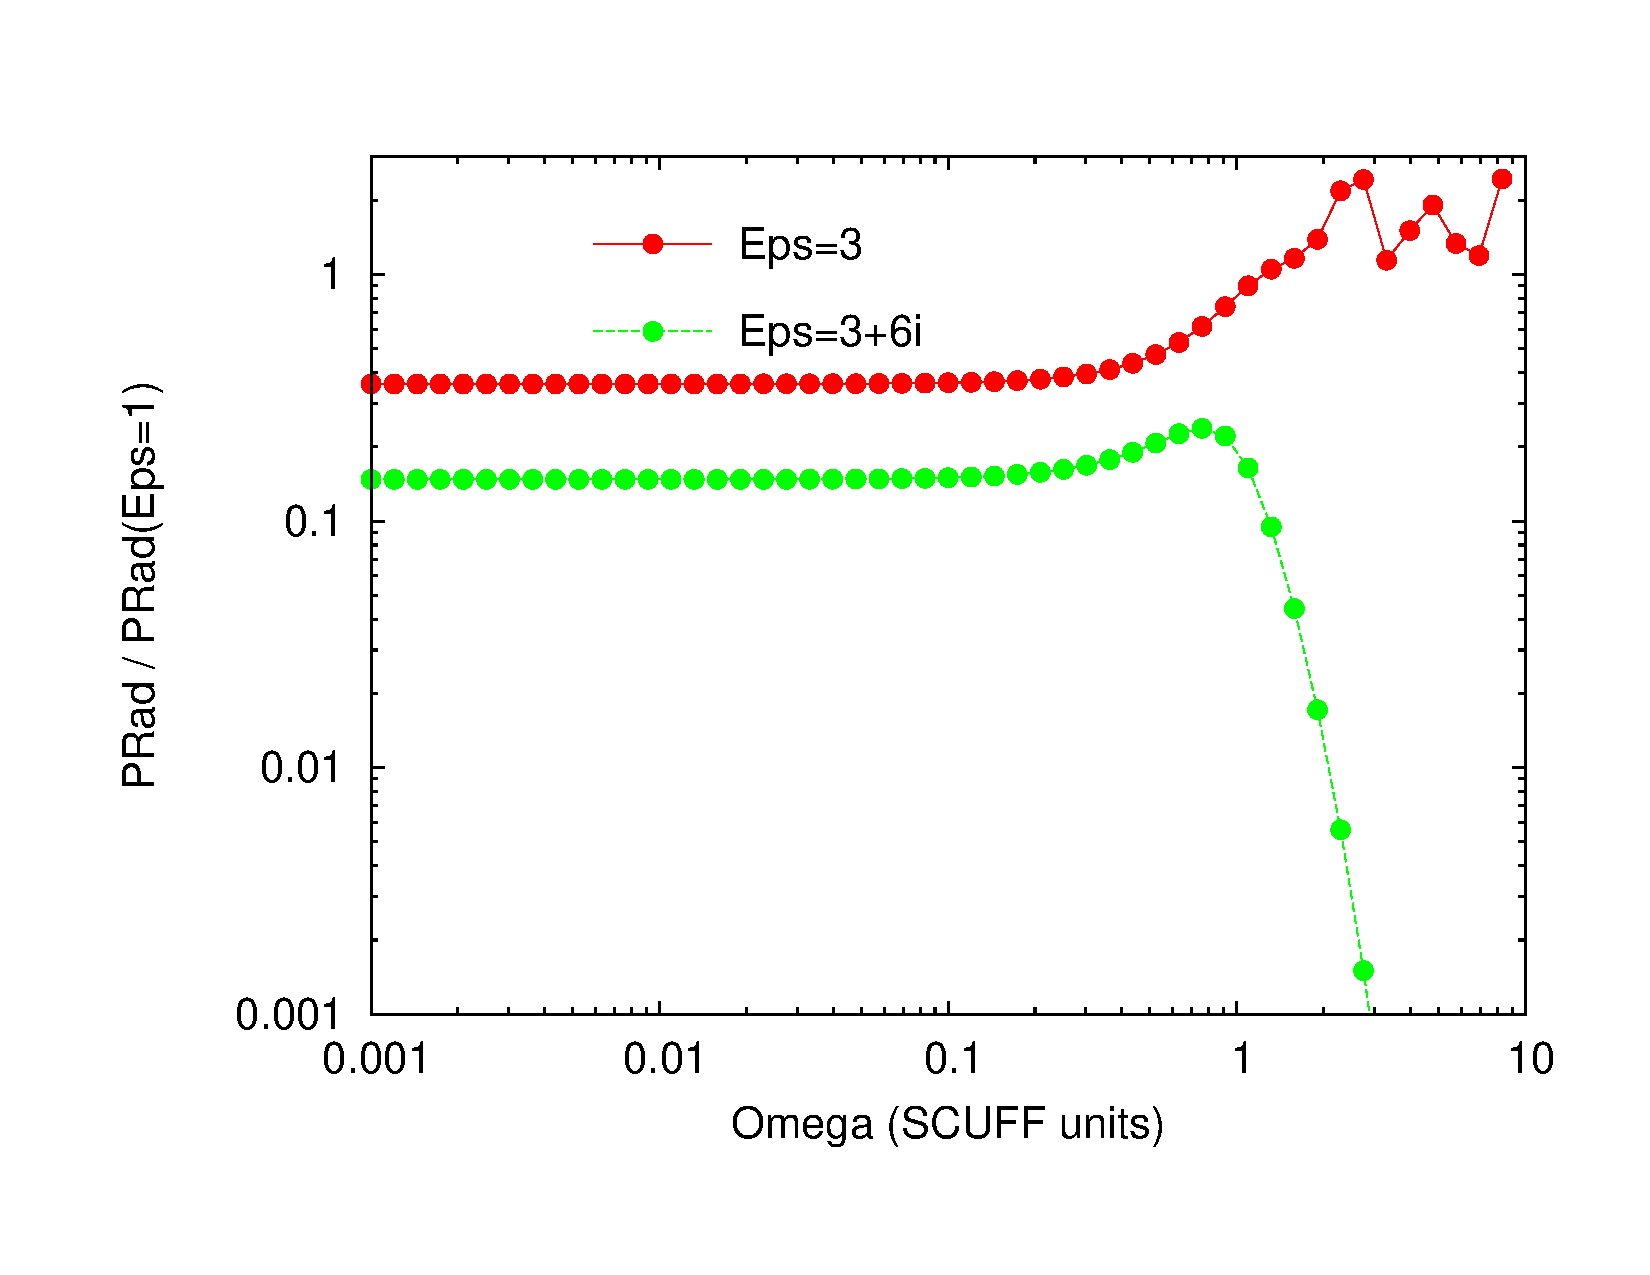
\includegraphics{PRadOverPRad0.pdf}}
\caption{Power radiated by a dipole at the center of a dielectric
sphere, normalized by the power radiated by a dipole in free space.}
\end{center}
\end{figure}
%####################################################################%

%%%%%%%%%%%%%%%%%%%%%%%%%%%%%%%%%%%%%%%%%%%%%%%%%%%%%%%%%%%%%%%%%%%%%%
%%%%%%%%%%%%%%%%%%%%%%%%%%%%%%%%%%%%%%%%%%%%%%%%%%%%%%%%%%%%%%%%%%%%%%
%%%%%%%%%%%%%%%%%%%%%%%%%%%%%%%%%%%%%%%%%%%%%%%%%%%%%%%%%%%%%%%%%%%%%%
\subsection{Sample stress-tensor force calculation}

The simplest incident-field configuration that gives rise to a
nonvanishing total force on the sphere is a superposition of 
$(1,0)$ and $(2,1)$ spherical waves, corresponding to coherent
dipole and quadrupole sources at the origin. Thus, in the
incident-field expansion (\ref{EIncExpansion}) we take
%%%%%%%%%%%%%%%%%%%%%%%%%%%%%%%%%%%%%%%%%%%%%%%%%%%%%%%%%%%%%%%%%%%%%%
\numeq{TwoNonvanishingPs}
{
 P_{(1,0)}=P_{(2,1)}=1,
 \qquad 
 P_\alpha=0 \text{ for all other }\alpha, 
 \qquad 
 Q_\alpha=0 \text{ for all }\alpha.
}
%%%%%%%%%%%%%%%%%%%%%%%%%%%%%%%%%%%%%%%%%%%%%%%%%%%%%%%%%%%%%%%%%%%%%%
The coefficients in expansions (\ref{EOutExpansion}, 
\ref{HOutExpansion}) for the fields outside the sphere 
are then similarly given by 
\numeq{TwoNonvanishingPs}
{
 C_{(1,0)}=C_{(2,1)}=\text{nonzero},
 \qquad 
 C_\alpha=0 \text{ for all other }\alpha, 
 \qquad 
 D_\alpha=0 \text{ for all }\alpha.
}
The actual values of $C_{(1,0)}$ and $C_{(2,1)}$, which
are less important for our immediate goals, are determined
by equation (\ref{CDAlpha}) for a specific frequency,
dielectric constant, and sphere radius. For example, 
for the particular case 
$\{ \omega, r_0, \epsilon\}
 =
 \{ \text{3 $\cdot$ 10$^{14}$ rad/sec},
    1\text{ $\mu$m},
    10
\}$
we find
$$ C_{(1,0)}=-0.558 + 0.760i, \qquad
   C_{(2,1)}= 0.100 + 0.001i.
$$

%%%%%%%%%%%%%%%%%%%%%%%%%%%%%%%%%%%%%%%%%%%%%%%%%%%%%%%%%%%%%%%%%%%%%%
%%%%%%%%%%%%%%%%%%%%%%%%%%%%%%%%%%%%%%%%%%%%%%%%%%%%%%%%%%%%%%%%%%%%%%
%%%%%%%%%%%%%%%%%%%%%%%%%%%%%%%%%%%%%%%%%%%%%%%%%%%%%%%%%%%%%%%%%%%%%%
\subsection{$x$-directed force density}

At a point $\vb x=(r_b, \Omega)$ on the surface of the bounding sphere
of radius $r_b$, the $x$-directed force per unit area is, from
(\ref{XForceFromEH}),
%====================================================================%
\begin{align*}
f_x(\vb x)
=\frac{\epsilon}{4}
  \bigg\{  &C^*_{10} C_{10} 
            \Big[ \vb M_{10}^*(\vb x) \bmc F_x(\Omega) \vb M_{10}(\vb x) 
                  + \vb N_{10}^*(\vb x) \bmc F_x(\Omega) \vb N_{10}(\vb x) 
            \Big]
\\
          +&C^*_{10} C_{21} 
            \Big[ \vb M_{10}^*(\vb x) \bmc F_x(\Omega) \vb M_{21}(\vb x) 
                  + \vb N_{10}^*(\vb x) \bmc F_x(\Omega) \vb N_{21}(\vb x)
            \Big]
\\
          +&C^*_{21} C_{10} 
            \Big[ \vb M_{21}^*(\vb x) \bmc F_x(\Omega) \vb M_{10}(\vb x) 
                  + \vb N_{21}^*(\vb x) \bmc F_x(\Omega) \vb N_{10}(\vb x)
            \Big]
\\
          +&C^*_{21} C_{21} 
            \Big[ \vb M_{21}^*(\vb x) \bmc F_x(\Omega) \vb M_{21}(\vb x) 
                  + \vb N_{21}^*(\vb x) \bmc F_x(\Omega) \vb N_{21}(\vb x)
            \Big]
  \bigg\}
\end{align*}
%====================================================================%

%%%%%%%%%%%%%%%%%%%%%%%%%%%%%%%%%%%%%%%%%%%%%%%%%%%%%%%%%%%%%%%%%%%%%%
%%%%%%%%%%%%%%%%%%%%%%%%%%%%%%%%%%%%%%%%%%%%%%%%%%%%%%%%%%%%%%%%%%%%%%
%%%%%%%%%%%%%%%%%%%%%%%%%%%%%%%%%%%%%%%%%%%%%%%%%%%%%%%%%%%%%%%%%%%%%%
\subsection{Total $x$-directed force}

The \textit{total} force is obtained from equation (\ref{TotalForce}):
\begin{equation}
 F_x = 
\frac{\epsilon_0}{4}
 \bigg\{
       C_{10}^* C_{21}
       \Big[ \Vmv{\vb M_{10}}{\bmc F_x}{\vb M_{21}}
            +\Vmv{\vb N_{10}}{\bmc F_x}{\vb N_{21}}
       \Big]
       + \text{CC}
 \bigg\}
\label{TotalForce2}
\end{equation}
where \text{CC} stands for ``complex conjugate.''
[The inner product here is defined by equation 
 (\ref{InnerProductDefinition}).]
With some effort, we compute
%%%%%%%%%%%%%%%%%%%%%%%%%%%%%%%%%%%%%%%%%%%%%%%%%%%%%%%%%%%%%%%%%%%%%%
$$
 \Vmv{\vb M_{10}}{\bmc F_x}{\vb M_{21}}
      +\Vmv{\vb N_{10}}{\bmc F_x}{\vb N_{21}}
 =-i\sqrt\frac{3}{10} \frac{1}{k^2}
$$
%%%%%%%%%%%%%%%%%%%%%%%%%%%%%%%%%%%%%%%%%%%%%%%%%%%%%%%%%%%%%%%%%%%%%%
and thus the total force (\ref{TotalForce2}) reads
\numeq{FxFinalSpecialCase}
{
 F_x = -\frac{\epsilon_0}{2k^2}\sqrt\frac{3}{10}\text{ Im }\Big(C_{10}^* C_{21}\Big)
}
%%%%%%%%%%%%%%%%%%%%%%%%%%%%%%%%%%%%%%%%%%%%%%%%%%%%%%%%%%%%%%%%%%%%%%
To make sense of the units here, suppose that field-strength
coefficients like $P,Q,C,D$ in (\ref{EIncExpansion}) and 
(\ref{EOutExpansion}) are measured in typical {\sc scuff-em}
units of V/$\mu $m, while $k$ is measured in units of 
inverse $\mu m$. Then the units of (\ref{FxFinalSpecialCase}) are

%%%%%%%%%%%%%%%%%%%%%%%%%%%%%%%%%%%%%%%%%%%%%%%%%%%%%%%%%%%%%%%%%%%%%%
\begin{align*}
 \text{units of (\ref{FxFinalSpecialCase})}
&=\frac{\epsilon_0 \cdot \text{V}^2 \cdot \mu\text{m}^{-2}}{\mu \text{m}^{-2}}
\intertext{Use $\epsilon_0=\frac{1}{Z_0 c}$ where $c$ is 
           the vacuum speed of light:}
&=\frac{1}{Z_0 c}\cdot \text{V}^2
\intertext{Use $Z_0=376.7$ V/A:}
&= \frac{ 376.7 \text{ V $\cdot$ A} }
        { 3\cdot 10^{14} \, \mu\text{m} \cdot \text{s}^{-1}}
\intertext{Now use 1 V$\cdot$ A=1 watt, 1 watt $\cdot$ 1 s = 1 joule,
           1 joule / 1 $\mu$m = 10$^6$ Newtons:}
&=1.26\cdot 10^{-6} \text{ Newtons.}
\end{align*}

%####################################################################%
\begin{figure}[H]
\begin{center}
\resizebox{\textwidth}{!}{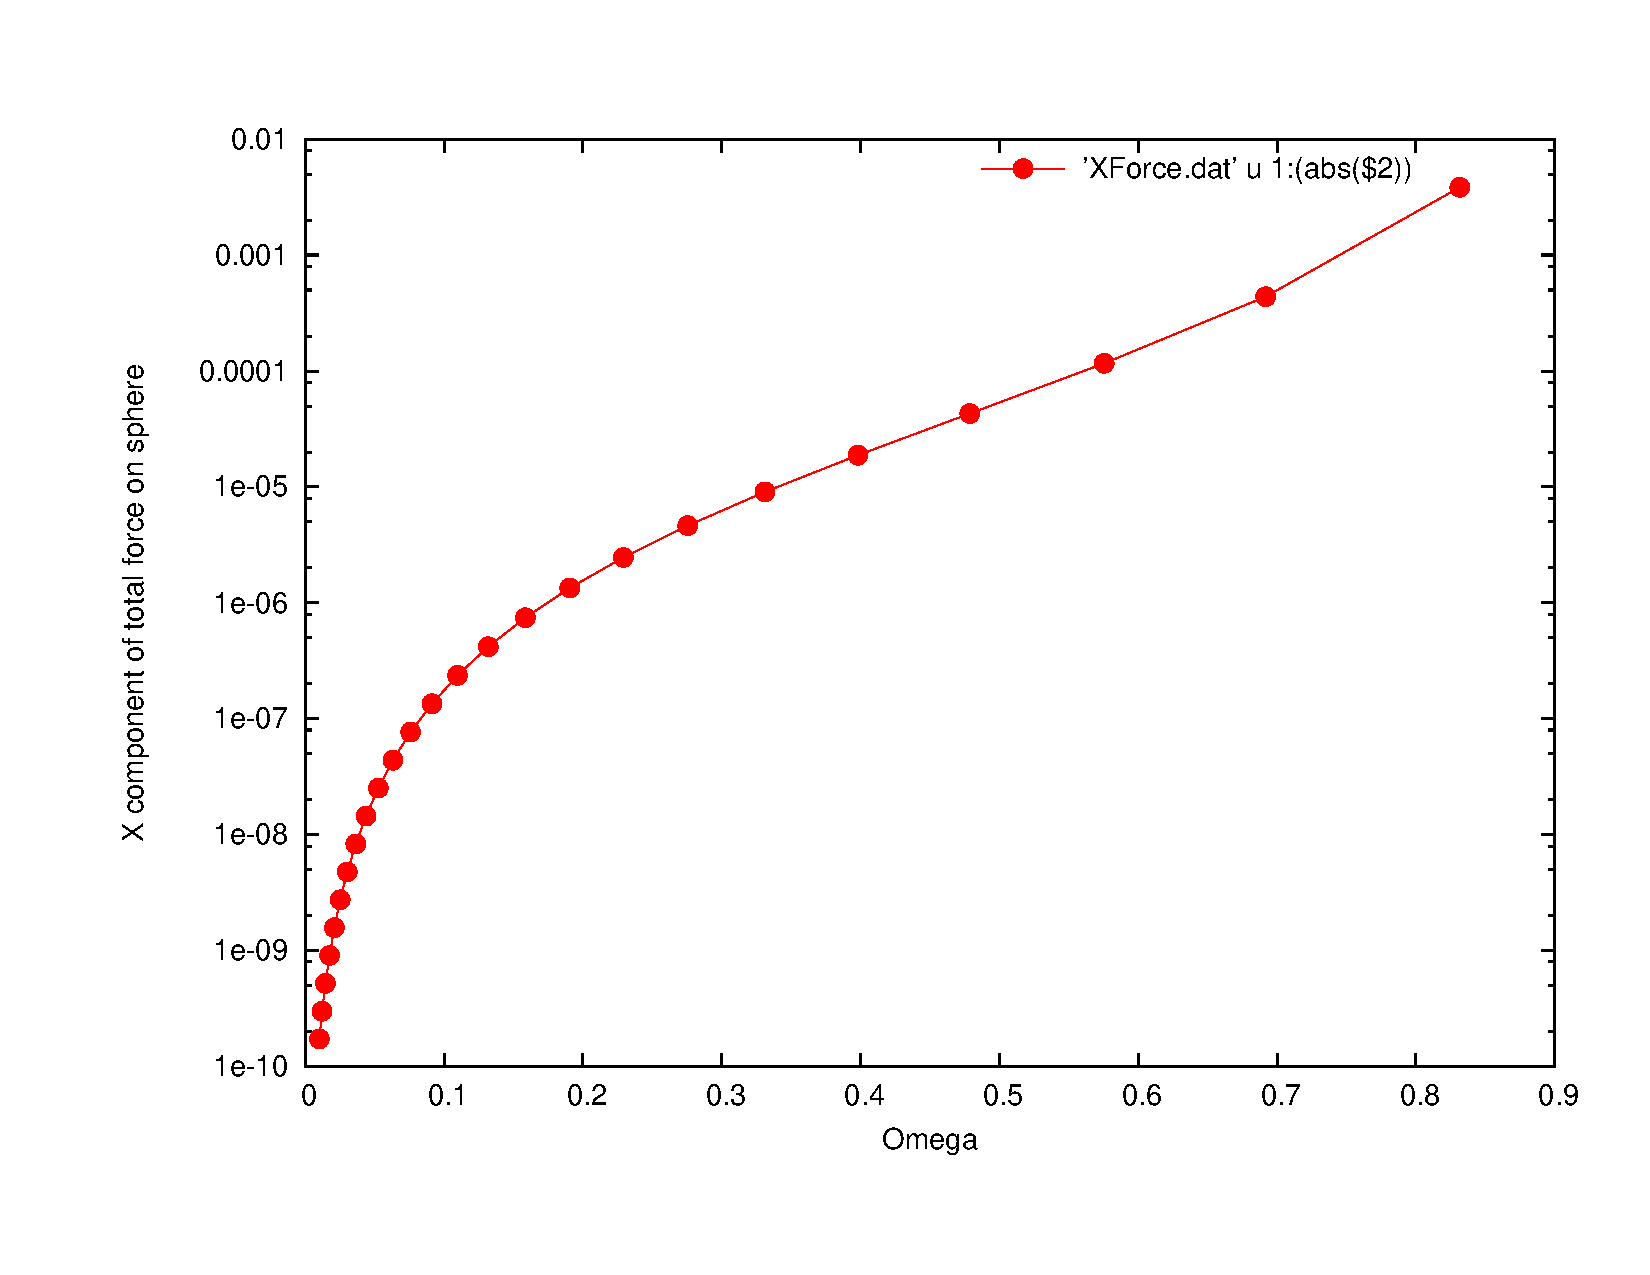
\includegraphics{ExactForce.pdf}}
\caption{$x$-component of total force on sphere irradiated from 
         within by an incident field of the form (\ref{EIncExpansion}) 
         with coefficients (\ref{TwoNonvanishingPs}).
        }
\label{TotalForce}
\end{center}
\end{figure}

%%%%%%%%%%%%%%%%%%%%%%%%%%%%%%%%%%%%%%%%%%%%%%%%%%%%%%%%%%%%%%%%%%%%%%
%%%%%%%%%%%%%%%%%%%%%%%%%%%%%%%%%%%%%%%%%%%%%%%%%%%%%%%%%%%%%%%%%%%%%%
%%%%%%%%%%%%%%%%%%%%%%%%%%%%%%%%%%%%%%%%%%%%%%%%%%%%%%%%%%%%%%%%%%%%%%
\newpage
\section{$\mb T$-matrix elements and surface currents}

The $\mb T$-matrix for a body relates the coefficients
of the outgoing spherical-wave expansion of the scattered
field to the coefficients of the regular spherical-wave
expansion of the incident field; thus, if we write
%====================================================================%
$$
 \vb E\sups{inc}  = \sum c\sups{inc}_\alpha \bmc W\sups{regular}_\alpha,
 \qquad
 \vb E\sups{scat} = \sum c\sups{scat}_\alpha \bmc W\sups{outgoing}_\alpha
$$
%====================================================================%
then the coefficient vectors are related by
%====================================================================%
$$\vb c\sups{scat} = \mb T \vb c\sups{inc}.$$
%====================================================================%
Individual $\mb T$-matrix elements have the significance
%====================================================================%
$$ \mb T_{\alpha\beta} = 
   \left\{\quad \parbox{0.45\textwidth}
          { coefficient of outgoing $\alpha$-type wave  \\
            due to irradiation by unit-amplitude incoming
            $\beta$-type wave.
          }\quad
  \right\}
$$
%====================================================================%
Now consider a scattering geometry irradiated by a unit-amplitude
regular wave, and let $\vb K$ and $\vb N$ be the electric and magnetic
surface currents induced by this excitation. The scattered field
is 
%====================================================================%
\begin{align}
 \vb E\sups{scat} &= ik Z \mb G \star \vb K + ik \mb C \star \vb N 
\nonumber
\intertext{ with $k$ and $Z$ the wavevector and (absolute) wave impedance
of the exterior medium. Insert the expansions (\ref{GCExpansions}):}
\vb E\sups{scat}(\vb x)
 &= -k^2 \sum_{\alpha}
    \left\{ Z \Inp{\bmc W\sups{reg}_\alpha}{\vb K}
             \bmc W\sups{out}_\alpha(\vb x)
          +\sigma_\alpha \Inp{\bmc W\sups{reg}_\alpha}{\vb N}
             \bmc W\sups{out}_{\overline{\alpha}}(\vb x)
   \right\}
\nonumber
\intertext{or, rearranging slightly,}
\vb E\sups{scat}(\vb x)
&= \sum_{\alpha}
   \underbrace{ -k^2
                \Big[  Z \inp{\bmc W\sups{reg}_\alpha}{\vb K}
                     -\sigma_{\overline{\alpha}} 
                         \inp{\bmc W\sups{reg}_{\overline{\alpha}}}{\vb N}
                \Big]
              }_{\mb T_{\alpha\beta}}\bmc W_{\alpha}\sups{out}(\vb x).
\label{TFromKN}
\end{align}
%====================================================================%
This yields a prescription for computing $\mb T$-matrix elements
directly from surface currents.
\end{document}
